\documentclass[12pt]{article}
\usepackage{paper, math}

\title{%
  Dynamic Treatment Effect Estimation with Interactive Fixed Effects and Short Panels\thanks{\acknowledgements}
}
\author{%
  \href{https://sites.google.com/msu.edu/nicholasbrown}{Nicholas Brown}\thanks{Queen's University, Economics Department (\href{mailto:n.brown@queensu.ca}{n.brown@queensu.ca})}
  \ and 
  \href{https://kylebutts.com/}{Kyle Butts}\thanks{University of Colorado Boulder, Economics Department (\href{mailto:kyle.butts@colorado.edu}{kyle.butts@colorado.edu})}
}
\date{\textsc{\today}}
\def\acknowledgements{
  We would like to thank Stephane Bonhomme, Brantly Callaway, Brian Cadena, Peter Hull, and Jeffrey Wooldridge, as well as seminar participants from the University of Georgia, Florida State University, Queen's University, the 2022 Midwest Econometrics Group, the CU Boulder Econometrics Brownbag, the 2023 CEA Annual Meeting, and the 2023 IAAE Annual Conference for their insightful questions and comments.
}

% Conditionally display thoughts (hide by switching to `\boolfalse`)
\boolfalse{INCLUDECOMMENTS}
\newcommand{\nick}[1]{\coauthorComment[Nick]{#1}}
\newcommand{\kyle}[1]{\coauthorComment[Kyle]{#1}}

\begin{document}

\maketitle
\vspace{-4mm}
\noindent\href{https://kylebutts.com/files/JMP.pdf}{[Most recent version]}

\begin{abstract}
  We study inference on dynamic average treatment effect parameters for staggered interventions when parallel trends are only valid conditional on an unobserved interactive fixed effects model. The interactive fixed effects model allows for units to select into treatment based on differential-exposure to macroeconomic shocks. We propose a general imputation-style estimator that is consistent in settings with few pre-treatment time periods and under arbitrary treatment effect heterogeneity. Our identification strategy allows for a wide set of factor-model estimators including principal components, common correlated effects, quasi-differencing, and more. % any first stage system of moments that controls the column space of the unobservable trends 
  %This result applies to data sets with either many or few pre-treatment time periods. 
  We also demonstrate the robustness of two-way fixed effects to certain parallel trends violations and describe how to test for its consistency. We investigate the effect of Walmart openings on local economic conditions and demonstrate that our methods ameliorate pre-trend violations commonly found in the literature.
  
  \par~\par\noindent
  \noindent{\color{asher} JEL Classification Number:} C13, C21, C23, C26
  \par
  \noindent{\color{asher} Keywords:} factor model, panel treatment effect, causal inference, fixed-T
  \par\vspace{-2.5mm}
\end{abstract}

\newpage


% ------------------------------------------------------------------------------
\section{Introduction}
% ------------------------------------------------------------------------------

For estimating the dynamic effects of a binary treatment in linear panel data models, difference-in-differences estimators are one of the most popular causal inference tools. In many empirical settings, treatment is assigned non-randomly based on trends in economic variables, and the parallel trends assumption required by difference-in-differences is not plausible. For example, in urban economics, place-based policies target places with worsening labor markets \citep{neumark2015place}, new apartments are built in appreciating neighborhoods \citep{asquith2021local,pennington2021does}, and firms opening new stores in growing economies \citep{basker2005job,neumark2008effects}. Estimation of treatment effects in this setting is confounded by the pre-existing economic trends. In many settings, though, it is reasonable to assume that the causes of these trends are due to larger economic forces and not location-specific shocks. Continuing our examples, the national decline of manufacturing caused targeted manufacturing hubs to be declining, consumer trends for walkable neighborhoods cause certain neighborhoods to become increasingly demanded, and national industry growth rates impact counties differentially. 

A recent growing literature models these kind of parallel trends deviations using an interactive fixed effects where there are common national shocks, but the exposure to the shock vary across locations. While interactive fixed effects relax the parallel trends assumptions relied on by difference-in-differences, the current literature requires long panels to estimate effects. Requiring long panels for estimation is often impractical because of (i) lack of data for many years of outcomes, (ii) strong assumptions like serially uncorrelated outcomes, or (iii) the presence of structural breaks, e.g. recessions or structural changes to the macroeconomy, rendering previous time periods uninformative about the current economy. This paper proposes a treatment effect estimator under the more general interactive fixed effect model that is robust to certain violations of parallel trends while remaining consistent in short panels and under heterogeneous treatment effects. 

We model untreated potential outcomes, $y_{it}(\infty)$, as an interactive fixed effect model
\begin{equation}\label{eq:untreated_po}
    y_{it}(\infty) = \bm{f}_t' \bm{\gamma}_i + u_{it},
\end{equation}
where $\bm{F}_t$ is a $p \times 1$ vector of unobservable factors, $\bm \gamma_i$ is a $p \times 1$ vector of unobservable factor loadings, and $\expec{u_{it}} = 0$ for all $(i,t)$.\footnote{We follow \citet{Callaway_Santanna_2021} and define the state of not receiving treatment in the sample as `$\infty$'. This is useful in settings with staggered treatment timing where potential outcomes are denoted by the period where a unit start treatments.} We can view, as we did in the above examples, the factors $\bm{F}_t$ as macroeconomic shocks with factor loadings $\bm \gamma_i$ denoting a unit's exposure to the shocks. Another possibility lets the $\bm \gamma_i$ represent time-invariant characteristics with a marginal effect on the outcome $\bm{F}_t$ that changes over time.\footnote{\citet{Ahn_Lee_Schmidt_2013} suggest a wage equation where $\bm \gamma_i$ are unobserved worker characteristics of an individual and $\bm{F}_t$ are their time-varying prices or returns to those characteristics. See \citet{Bai_2009} for a collection of economic examples that justify the inclusion of a factor structure.} Note that this model nests the standard two-way error model when $\bm{F}_t' = (\lambda_t, 1)$ and $\bm \gamma_i' = (1, \mu_i)$; that is, $\bm{F}_t' \bm \gamma_i = \lambda_t + \mu_i$. The interactive structure allows for more general patterns of unobserved heterogeneity. Importantly, we allow for treatment to be correlated with a unit's exposure to macroeconomic shocks via their factor loadings $\bm{\gamma}_i$. 

For a concrete example, our empirical application focuses on estimating the effect of Walmart store openings on county-level employment. Estimation of a standard two-way fixed effect event-study model suggests that Walmart opened stores in counties that had higher retail employment growth prior to the opening (e.g. \citet{neumark2008effects}). In \autoref{fig:walmart_retail}, we present an event-study graph and overlay a line of best fit on the pre-treatment estimates. That the line is positive sloping and the estimates are different from zero at the 5\% level suggests that estimated positive impacts are due to pre-existing trends rather than the effect of Walmart per se. However, there seems to be a discrete jump when the Walmart opened. The goal then is to remove these pre-existing trends to isolate the treatment effect. It is plausible to assume that during their period of mass expansion, Walmart selected appealing locations based on their local demographic background and national economic trends, while ignoring transitory local economic shocks. Our framework allows this type of selection mechanism and effectively `controls' for these pre-existing trends in outcome.

Our main treatment effect identification result only requires consistent estimates of the column space of $\bm{F}_t$. Using the estimated factors, we compute a matrix that projects the pre-treatment outcomes onto the estimated post-treatment factors, imputing the untreated potential outcome for treated units. Averaging over the difference between the post-treatment observed outcomes and the estimated untreated potential outcomes gives a consistent estimator of average treatment effects. In specifications that include the two-way error model, we show how to explicitly remove the additive fixed effects with a double-demeaning transformation that maintains the common factor structure across treated groups and the never-treated group.

There are two major benefits of our general identification argument. First, consistent estimation of $\bm{F}_t$ is possible through a variety of approaches, such as quasi-differencing \citep{Ahn_Lee_Schmidt_2013,Callaway_Karami_2020}, common correlated effects \citep{pesaran2006estimation,Westerlund_Petrova_Norkute_2019}, or principal components \citep{Bai_2009,Fan_2016,Westerlund_2020,Chan_and_Kwok_2022}. These techniques allow the user to tailor their factor estimator to the specific data and problem under consideration, including how many pre-treatment time periods are available. Our identification result provides a recipe for using any consistent estimator of the factors to estimate treatment effects, opening up the large factor-model literature for causal inference methods. Second, our imputation method allows researchers to graph the estimated counterfactual untreated potential outcomes and the observed outcomes for treated units as a visual check for the parallel trends assumption, similar to a synthetic control plot.

We derive asymptotic properties of an imputation estimator with factor proxies that contain the true unobserved factors in their column space. The resulting estimator takes the form of a generalized method of moments (GMM) estimator, which allows estimation and inference via common statistical software. It is also consistent when the number of pre-treatment time periods is small.\footnote{Deriving the asymptotic distribution of treatment effects using large-$T$ factor estimators is left for future work.} One advantage of this estimator is that we can form statistical tests for the consistency of the two-way fixed effects (TWFE) estimator. These tests are practically useful since difference-in-differences is simple to implement. 

\subsection*{Relation to Literature}

Recent work has proposed `imputation' estimators for treatment effects using non-treated and pre-treatment observations to `impute' the untreated potential outcomes for the post-treatment observations \citep[e.g.][]{Borusyak_Jaravel_Spiess_2021,Gardner_2021,Wooldridge_2021}. However, these approaches only allow for level fixed effects and preclude interactions like in equation (\ref{eq:untreated_po}). \citet{Borusyak_Jaravel_Spiess_2021} allow a structure similar to equation \eqref{eq:untreated_po} but requires the the factors $\bm{F}_t$ be observed. We generalize these techniques by proposing an estimator that imputes the untreated potential outcomes under the more general (\ref{eq:untreated_po}) with unobserved interactive effects.

Current estimators that allow for selection based on a factor model either require (i) the number of time periods available is large, e.g. synthetic control \citep{abadie2021using}, factor-model imputation \citep{Xu_2017,Gobillon_Magnac_2016}, and the matrix completion method  \citep{Athey_et_al_2021,fernandez2021low}; or (ii) that an individual's error term $u_{it}$ is uncorrelated over time \citep{Imbens_Kallus_Mao_2021}.\footnote{\citet{Imbens_Kallus_Mao_2021} allow correlation within the post- and pre-treatment sets of the idiosyncratic errors, but assume independence between the two sets. This assumption is still strong in a static modeling context.} Both of these restrictions are non-realistic in many applied microeconomic data sets where the number of time periods is much smaller than the number of units and serial correlation of shocks is expected. Further, large-$T$ estimators often place restrictions on the dynamic heterogeneity of treatment. Our method requires neither large $T$ nor error term restrictions, but can still accommodate large-$T$ and unit-heterogeneous estimation strategies.

Our work contributes to an emerging literature on adjusting for parallel trends violations in short panels. \citet{freyaldenhoven2019pre} propose a similar instrumental variable type estimator in the presence of time-varying confounders. Their results rely importantly on homogeneous treatment effects. Their simulations show that heterogeneous treatment effects bias their estimates severely, while our estimator allows for arbitrary time heterogeneity. The most similar paper to our current approach is \citet{Callaway_Karami_2020}, who also allow for heterogeneous effects in short panels. They prove identification using a similar strategy to QLD and instrumental variables and derive asymptotic normality assuming the number of time periods is fixed. They require time-invariant instruments whose effects on the outcome are constant over time. Their instruments are valid for the QLD estimator in our application, but we also allow for time-varying covariates as instruments. They do not provide a general identification scheme like ours and so their results do not readily extend to other estimators like principal components or common correlated effects.

The rest of the paper is divided into the following sections: Section \ref{sec:theory} describes the theory behind our methods and presents identification results of the group-specific dynamic treatment effect parameters. Section \ref{sec:estimation} provides the main asymptotic theory for a particular QLD estimator. We also discuss practical concerns for practitioners. We include a small Monte Carlo experiment in Section \ref{sec:simulations} to examine the finite-sample performance of our estimator. Finally, Section \ref{sec:application} contains our application and Section \ref{sec:conclusion} leaves with some concluding remarks. 


% ------------------------------------------------------------------------------
\section{Model and Identification} \label{sec:theory}
% ------------------------------------------------------------------------------

We assume a panel data set with units $i = 1,\dots, N$ and periods $t = 1, \dots, T$. Treatment turns on in different periods for different units; we denote these groups by the period they start treatment. For each unit, we define $G_i$ to be unit $i$'s group with possible values $\{ g_1, \dots, g_G \} \equiv \mathcal{G} \subseteq \{ 2, \dots, T \}$. We follow \citet{Callaway_Santanna_2021} and denote $G_i = \infty$ for units that never receive treatment. We assume that $0 < P(G_i = g) < 1$ for all $g \in \mathcal{G} \cup \{ \infty \}$, so that the number of individuals in each group and the never-treated group grow with $N$. Treated potential outcomes are a function of group-timing, which we denote $y_{it}(g)$. For treatment indicators, we define the vector of treatment statuses $\bm d_{i} = (d_{i1},...,d_{iT})$ where $d_{it} = \mathbf{1}(t \geq G_i)$ and the indicator $D_{ig} = \mathbf{1}(G_i = g)$ if unit $i$ is a member of group $g$. Let $T_0 = \min_j \{ g_j \} - 1$ be the last period before the earliest treatment adoption. 

% We also introduce some matrix notation. For a vector $\bm x$ of length $T$, we use the subscript $\bm x_{t < g}$ to denote the first $g - 1$ elements and $\bm x_{t \geq g}$ to refer to the last $T - g + 1$ elements. This holds similarly for the rows of a matrix $\bm X$. 

Following \citet{Callaway_Santanna_2021}, we aim to estimate group-time average treatment effects on the treated:
\begin{equation}
  \ATT(g,t) = \tau_{gt} \equiv \expec{y_{it}(g)}{G_i = g} - \expec{y_{it}(\infty)}{G_i = g}
\end{equation}
These quantities represent the average effect of treatment at time $t$ for units that start treatment in period $g$ for $t \geq g$. It is trivial to estimate other averages as well in our framework, including averaging over all post-treatment observations to estimate an overall $\ATT$, and averaging over $(i,t)$ where $t - G_i = \ell$ to estimate event-study estimands $\ATT^\ell$'s. We discuss these and other extensions from \citet{Callaway_Santanna_2021} in Section \ref{sec:estimation}.

We now state our main identifying assumptions.
\begin{assumption}[\textbf{Sampling}]\label{asm:sampling}
The random vectors $\{ (\bm d_i, \bm \gamma_i, \bm u_i) \}$ are randomly sampled from an infinite population and has finite moments up to the fourth order. $\blacksquare$
\end{assumption}

\begin{assumption}[\textbf{Untreated potential outcomes}]\label{asm:untreated_po}
The untreated potential outcomes take the form
\begin{equation*}
  y_{it}(\infty) = \bm{F}_t' \bm \gamma_i + u_{it}
\end{equation*}
where $\expec{u_{it}}{\bm d_i, \bm \gamma_i} = 0$ for $t = 1,...,T$. $\blacksquare$
\end{assumption}

\begin{assumption}[\textbf{No anticipation}]\label{asm:no_anticipation}
For all units $i$ and groups $g \in \mathcal{G}$, $y_{it} = y_{it}(\infty)$ for $t < g$. $\blacksquare$ % Or, less strictly, we require $\expec{y_{it}}{G_i = g} = \expec{y_{it}(\infty)}{G_i = g}$ for $t < g$.
\end{assumption}

Assumption \ref{asm:untreated_po} imposes a factor-model for the untreated potential outcomes. The Online Appendix discusses the inclusion of covariates and the subsequent relaxation of assumption \ref{asm:untreated_po}. We allow for heterogeneous and dynamic treatment effects of any form, i.e. $y_{it}(g) = \tau_{igt} + y_{it}(\infty)$. We also allow arbitrary serial correlation among the idiosyncratic errors.\footnote{This condition may need to be strengthened for inference when $T \rightarrow \infty$.} We assume the common factors $\bm{F}_t$ are nonrandom parameters and the number of factors $p$ is fixed in the asymptotic analysis. 

Assumption \ref{asm:untreated_po} is more general than the standard difference-in-differences parallel trend assumption since we include the factor structure in our potential outcome model. In particular, it assumes that the error term is uncorrelated with treatment status \emph{after} controlling for the factor loadings. Treatment can still be correlated with contemporaneous shocks so long as the shocks, but not necessarily the exposure to them, are `common' across the sample. For example, our identification strategy is valid if workers select into a job training program based on their exposure (or adaptability) to macroeconomic productivity shocks. 

The two-way error model cannot generally accommodate differential exposure.\footnote{The following derivation is also shown in \citet{Callaway_Karami_2020}, but we are repeating it here for exposition.} In the more general factor model and \autoref{asm:untreated_po}, changes in untreated potential outcomes are given by
\begin{equation*}
  \expec{y_{it}(\infty) - y_{it-1}(\infty)}{G_i = g} = \lambda_t + (\bm{F}_t - \bm{F}_{t-1})' \expec{\bm \gamma_i}{G_i = g}
\end{equation*}
Unless either (i) the factor loadings have the same mean across treatment groups, $\expec{\bm \gamma_i}{G_i = g} = \expec{\bm \gamma_i}$, or (ii) the factors are time-invariant, then the standard parallel trends assumption that the group $g$ and the never-treated group follow common trends would not hold. If either of the two cases hold for all $g$ and $t$, the two-way error model is correctly specified.\footnote{We explicitly prove this result later.} However, these are knives edge cases which are not the focus of the paper. Our Assumption \ref{asm:untreated_po} allows for the factor loadings to be correlated with treatment timing and opens up treatment effect estimation for a much broader set of empirical questions.

The key econometric challenge lies in that we do not observe $y_{it}(\infty)$ whenever $d_{it} = 1$. Our goal is to consistently estimate $\expec{y_{it}(\infty)}{G_i = g}$ under equation (\ref{eq:untreated_po}) to consistently estimate group-time average treatment effects. \citet{Gardner_2021}, \citet{Wooldridge_2021}, and \citet{Borusyak_Jaravel_Spiess_2021} implicitly rely on this insight in studying the two-way error model. 

Prior attempts at estimating average treatment effects in a factor-model setting focus on finding conditions that allow for estimation of $\bm \gamma_i$ and $\bm{F}_t$ jointly as in \citet{Gobillon_Magnac_2016} and \citet{Xu_2017}, or a generalized version of a factor model as in \citet{arkhangelsky2021synthetic}. These techniques require the number of pre-treatment periods to grow to infinity and often place restrictions on both the dynamics of the treatment effects' distribution and the serial dependence among the idiosyncratic errors. Instead, we pursue identification noting that 
\begin{equation}\label{eq:untreated_cond_expectation}
\expec{y_{it}(\infty)}{G_i = g} = \bm{F}_t' \expec{\bm \gamma_i}{G_i = g}
\end{equation}
Therefore, we only need to estimate the \emph{average} of the factor loadings among a treatment group, which we can always do even with a small number of post-treatment time periods. We can then accommodate either a large or small number of pre-treatment periods and allow for estimation using a broad range of known strategies.

\subsection{\texorpdfstring{$\ATT(g,t)$}{ATT(g,t)} Identification}\label{sec:ATT_identification}

We begin by describing the intuition behind our identification result. Consider a unit subject to treatment at time $g$. Define $\bm y_{i,t<g}$ and $\bm y_{i,t\geq g}$ as respectively the first $(g-1)$ and last $(T-g+1)$ outcomes for unit $i$. Define $\bm{F}$ to be the matrix of factor shocks with rows given by $\bm{F}_t$. We similarly define $\bm{F}_{t < g}$ and $\bm{F}_{t \geq g}$ as the first and last rows of matrix $\bm{F}$. Equation \eqref{eq:untreated_cond_expectation} implies
\begin{equation}
  \expec{\bm y_{i,t < g}(\infty)}{ \bm G_i = g} = \bm{F}_{t < g} \expec{\bm \gamma_i}{\bm G_i = g}
\end{equation}
If the factors were observed, we could consistently estimate the mean values of the $p$-vector of average factor loadings for treated group $G_i = g$. More formally, if $\text{Rank}(\bm{F}_{t < g}) = p$, the coefficient from the population regression of $\expec{y_{i,t < g}(\infty) }{ G_i = g}$ on $\bm{F}_{t < g}$ is $\expec{\bm \gamma_i}{G_i = g}$. Equation \eqref{eq:untreated_cond_expectation} also gives us 
\begin{equation}
  \expec{\bm y_{i,t \geq g}(\infty)}{ \bm G_i = g} = \bm{F}_{t \geq g} \expec{\bm \gamma_i}{\bm G_i = g}
\end{equation}
for the post-treated outcomes. Because we assume $\bm{F}$ is known (for now), we can predict $\expec{\bm y_{i,t}}{G_i = g}$ for $t \geq g$ by multiplying $\bm{F}_t$  by the OLS estimate from the prior regression. We then obtain $\expec{y_{it}(\infty)}{G_i = g}$ for the post-treatment outcomes, which we can subtract from $y_{i t}$ and average over the respective sample to obtain $\text{ATT}(g,t)$. 

We now define a useful matrix function for a more formal derivation of our main result. Given matrices $\bm X_1$ and $\bm X_0$ that are respectively $n \times k$ and $m \times k$, suppose $\text{Rank}( \bm X_0) = k$. We define the \emph{imputation matrix} 
\begin{equation}
  \bm P(\bm X_1, \bm X_0) \equiv \bm X_1 (\bm X_0' \bm X_0)^{-1} \bm X_0'
\end{equation}
This matrix takes a similar form to a projection matrix but ``imputes" the fitted values from regressing on $\bm X_0$ onto a different matrix $\bm X_1$. \citet{Gardner_2021} and \citet{Borusyak_Jaravel_Spiess_2021} implicitly uses the imputation matrix for an additive error model where $\bm X_1$ is the matrix of unit and time fixed effects and $\bm X_0$ is $\bm X_1$ with rows of zero whenever $d_{it} = 1$. When applying this matrix of factors to our outcomes, the post-treatment factors are multiplied by the factor loadings from the pre-treatment observations. In particular, we impute $y_{it}(\infty)$ by $\bm P(\bm{F}_{t}', \bm{F}_{t < g}) \bm y_{i,t < g}$ for $G_i = g$, similar to the bridge function identification scheme in \citet{Imbens_Kallus_Mao_2021}. However, because we only need a conditional mean assumption, we can allow arbitrary correlation between the idiosyncratic errors. 

The next theorem provides our main identification result:
\kyle{We haven't defined $\bm{\theta}$ yet here, so I just used $\bm{F}^*$.}
\begin{theorem}\label{theorem:ATT_identification}
  Suppose $\bm{F}$ is known and $\text{Rank}(\bm{F}_{t \leq T_0}) = p$. Under Assumptions \ref{asm:sampling}, \ref{asm:untreated_po}, and \ref{asm:no_anticipation} for all $g \in \mathcal{G}$,
  \begin{equation}\label{eq:ATT_moments}
    \ATT(g,t) = \expec{y_{it} - \bm P(\bm{F}_{t}', \bm{F}_{t < g}) \bm y_{i,t < g}}{G_i = g}
  \end{equation}
  for $t \geq g$. 

  Moreover, let $\bm{F}^*$ be a full rank $T \times m$ matrix where $m < T_0$ and $\bm{F} \in \text{col}(\bm{F}^*)$, the column space of $\bm{F}^*$. Then the imputation matrix is invariant to $\bm{F}^*$
  \begin{equation}
    \bm P(\bm{F}_t^{*'}, \bm{F}^*_{t < g}) \bm{F}_{t < g} \bm \gamma_i = \bm{F}_t' \bm \gamma_i
  \end{equation}
  $\blacksquare$
\end{theorem}

All proofs are contained in the Online Appendix. Theorem \ref{theorem:ATT_identification} shows that we can identify the ATTs if we know the factor matrix. The second part of the theorem suggests that any rotation of the true factor matrix, $\bm{F}$, can be used in the imputation matrix. This is important because it is well understood that $\bm{F}_t$ and $\bm{\gamma}_i$ are not separately identified \citep{Ahn_Lee_Schmidt_2013,Xu_2017}. All of the estimators discussed so far can at best approximate the column space of the factors because both $\bm{F}_t$ and $\bm \gamma_i$ are unobserved. The second part of the theorem shows that our identification scheme allows for this class of estimators. 

\autoref{theorem:ATT_identification} shows we can apply these conclusions to any interactive fixed effects estimator that achieves consistency by asymptotically spanning the factor space. Examples include the principal components estimator of \citet{Bai_2009}\footnote{The PC estimator in \citet{Bai_2009} requires $T \rightarrow \infty$ for asymptotic normality. \citet{Westerlund_2020} provides conditions under which the PC estimator is fixed-$T$ consistent. Regardless, the identification strategy still holds.}, the common correlated effects estimator of \citet{pesaran2006estimation}\footnote{The CCE factor proxies do not converge to a full rank matrix. However, \citet{Westerlund_Petrova_Norkute_2019} show that the residual maker matrix is consistent for the space orthogonal to the factors due to an implicit normalization. See \citet{Brown_Butts_Westerlund_2023} for a proof of asymptotic normality in our setting under typical CCE assumptions.}, the differencing techniques of \citet{Ahn_Lee_Schmidt_2001,Ahn_Lee_Schmidt_2013}, \citet{Callaway_Karami_2020} and \citet{Brown_2022}, or the internally generated instruments of \citet{Juodis_Sarafidis_2022} or \citet{Cui_et_al_2022}. As long as the factors are consistently estimated using the control sample, dynamic $\ATT$s are identified as in Theorem \ref{theorem:ATT_identification}, regardless of the normalization used for estimation. In fact, we do not even require the factors to be full rank, though this assumption is typically made in practice. 

To present a general framework for the estimation of the factors, we formally present the identifying assumptions needed for factor space estimators:
\begin{assumption}\label{asm:factor_identification}
  There exists a $q \times 1$ vector of parameters $\bm{\theta}$ and a $T \times m$ function $\bm{F}(\bm{\theta})$ such that the following conditions hold:
  \begin{enumerate}[(i)]
    \item For some full-rank matrix $\bm{A}$, $\bm{F}(\bm{\theta}) \bm{A} = \bm{F}$ where $\text{Rank}(\bm{F}(\bm{\theta})) = m < T_0$ 
    \item There is a $s \times 1$ vector of moment functions $\bm g_{i\infty}(\bm{\theta})$ such that 
    \begin{equation}\label{eq:factor_moments}
      \expec{\bm g_{i\infty}(\bm{\theta})}{G_i = \infty} = \bm 0
    \end{equation}
    
    \item Let $\bm D_{\infty} = \expec{\nabla_{\bm{\theta}} \bm g_{i \infty}(\bm{\theta})}{G_i = \infty}$. Then $\text{Rank}(\bm D_{\infty}) = q$.
    \item $\expec{\bm g_{i \infty}(\bm{\theta}) \bm g_{i \infty}(\bm{\theta})'}{G_i = \infty}$ is positive definite. 
  \end{enumerate}
\end{assumption}
Part (i) implies that the estimated factors can be reduced to a finite dimension of estimable parameters. The matrix $\bm A$ is the full rank linear rotation that turns $\bm{F}(\bm{\theta})$ into $\bm{F}$. For the example estimators expressed above, $\bm{F}(\bm{\theta})$ asymptotically spans the unknown factors, $\bm{F}$. Parts (ii)-(iv) imply the parameters $\bm{\theta}$ are identified and consistently estimable. The parameters $\bm{\theta}$ themselves are often the result of an underlying normalization like in \citet{Bai_2009}, \citet{Ahn_Lee_Schmidt_2013}, \citet{Juodis_Sarafidis_2022}, and \citet{Callaway_Karami_2020}. Sometimes they are population moments estimated by cross-sectional averages like in \citet{Westerlund_Petrova_Norkute_2019} and \citet{Brown_Schmidt_Wooldridge2021}. 

% \citet{Chan_and_Kwok_2022} propose a principal components difference-in-differences estimator for unit-specific treatment effects, ruling out dynamic effects because of the large time series assumed in the asymptotic arguments. Our results show that estimation of the factors can be carried out using untreated observations and then applied to any post-treatment period for a time-specific ATT. This result relaxes their time-homogeneity assumption while also allowing for empirical examples where there are many time observations.
Assumption \ref{asm:factor_identification} is written with fixed-$T$ estimation and inference in mind. As mentioned before, accommodating general principal components estimation requires additional restrictions, as well as a large time series in the pre-treatment periods. However, the general identification result is the same and our estimator is still valid for estimating dynamic effects in the post-treatment period. Further research should explicitly derive the large-$T$ properties of our estimator using principal components in the first stage. 

\begin{remark}\label{remark:QLD}
A leading example of a set of moment equations for factor-space estimation is the Quasi-long Differencing (QLD) estimator of \citet{Ahn_Lee_Schmidt_2013} (ALS). ALS propose a QLD transformation given by 
\begin{equation}
  \bm H(\bm \upsilon) = (\bm I_{T-p}, \bm \Upsilon)
\end{equation}
where $\bm \Upsilon$ is a $(T-p) \times p$ matrix of unrestricted parameters and $\bm \upsilon = \text{vec}(\bm \Upsilon)$. They normalize the factors as 
\begin{equation}
  \bm{F}(\bm \upsilon) = 
  \begin{pmatrix}
    \bm \Upsilon\\
    -\bm I_p
  \end{pmatrix}
\end{equation}
so that $\bm H(\bm \upsilon) \bm{F} \bm \gamma_i = \bm 0$ by construction. We modify their proposed moment conditions to use just the never-treated group:
\begin{equation}
  \expec{g_{i\infty}(\bm{\upsilon})}{D_{i\infty} = 1} = \expec{\bm w_i \otimes \bm H(\bm \upsilon) \bm y_i}{D_{i\infty} = 1} = \bm 0
\end{equation}
where $\bm w_i$ is a vector of instruments that are exogenous with respect to the idiosyncratic error in \autoref{asm:untreated_po} but correlated with $\bm \gamma_i$. We discuss the choice of instruments $\bm w_i$ in more practical terms in \autoref{sec:application}.

While both approaches are valid in the first stage of our setting, we use the \citet{Ahn_Lee_Schmidt_2013} estimator because it is more general than \citet{Callaway_Karami_2020}. For one, they allow for a larger set of instruments. One identification strategy proposed by \citet{Callaway_Karami_2020} requires time-invariant covariates whose effects on $y_{it}$ are independent of time, meaning the researcher must decide which of the time-invariant observables have constant effects on the outcome. \citet{Ahn_Lee_Schmidt_2013} can allow for arbitrary time effects on covariates while still using those covariates as instruments. \citet{Ahn_Lee_Schmidt_2013} also give a road map to estimation based on weakly exogenous covariates that allows for dynamic modeling. This aspect of the estimator is left for future research.
$\blacksquare$
\end{remark}

\kyle{Discussion of selecting $p$}


\subsection{Two-Way Error Model}

We now demonstrate how to explicitly nest the standard two-way error model. While this structure is a special case of the factor model studied above, we consider the special case for two main reasons. First, eliminating the additive effects saves degrees of freedom to estimate the factor models; it may also provide efficiency by reducing the burden on first-stage factor estimators. Second, a thorough study of the additive model will provide insight into the link between TWFE estimation and more complicated and computationally involved factor model estimation. It will also allow us to show when TWFE estimation is consistent in the presence of interactive fixed effects. 

We first note that care must be taken when eliminating additive effects so that the overall factor structure is preserved. The methods in \citet{Borusyak_Jaravel_Spiess_2021}, \citet{Gardner_2021}, and \cite{Wooldridge_2021} that estimate the additive effects using the untreated sample will not maintain a common factor structure. For example, consider the first order conditions from the regression of $(1 - d_{it})y_{it}$ on unit and time effects. The estimators for the unit effect of a unit treated at time $g$ and a never-treated unit respectively satisfy
\begin{align}
  &\sum_{t = 1}^{g-1} (y_{it} - \widehat{\lambda}_t - \widehat{\mu}_i) = 0\\
  &\sum_{t = 1}^T (y_{it} - \widehat{\lambda}_t - \widehat{\mu}_i) = 0
\end{align}
The control sample will remove more time averages than in every treated sample, meaning the factors are demeaned using different subsamples. As such, the transformed factors are not equal across groups and so we cannot then use the control sample to estimate the factors for the treated samples. 

We first define the following averages for the purpose of removing the additive effects:
\begin{gather}
  \overline{y}_{\infty , t} = \frac{1}{N_{\infty}} \sum_{i = 1}^N D_{i \infty} y_{it} \\
  \overline{y}_{i,t\leq T_0} = \frac{1}{T_0} \sum_{t = 1}^{T_0} y_{it} \\
  \overline{y}_{\infty, t < T_0} = \frac{1}{N_{\infty} T_0} \sum_{i = 1}^N \sum_{t = 1}^{T_0} D_{i \infty} y_{it}
\end{gather}
where $\overline{y}_{\infty , t}$ is the cross-sectional averages of the never-treated units for period $t$, $\overline{y}_{i,t\leq T_0}$ is the time-averages of unit $i$ before any group is treated, and $\overline{y}_{\infty, t < T_0}$ is the total average of the never-treated units before any group is treated.

We then perform all estimation on the residuals $\tilde{y}_{it} \equiv y_{it} - \overline{y}_{\infty, t} - \overline{y}_{i,t < T_0} + \overline{y}_{\infty, t < T_0}$. These residuals are reminiscent of the usual TWFE residuals, except we carefully select this transformation to accomplish two things. First, this transformation leaves the treatment dummy variables unaffected to prevent problems with negative weighting when aggregating heterogeneous treatment effects \citep{Goodman-Bacon_2021,Borusyak_Jaravel_Spiess_2021}. Second, it preserves a common factor structure for all units and time periods\footnote{Such a transformation should not be used when considering the common correlated effects estimator because it would violate the CCE rank condition. See \citet{Brown_Butts_Westerlund_2023}.}. The TWFE imputation estimator of \citet{Gardner_2021}, \citet{Wooldridge_2021}, and \citet{Borusyak_Jaravel_Spiess_2021} would not share this property because they estimate $\mu_i$ and $\lambda_t$ based on the full sample $d_{it} = 0$, while we use a specific subsample.

This result is summarized in the following lemma:
\begin{lemma}\label{lemma:twfe_residuals}
  $\expec{\tilde{y}_{it}}{G_i = g} = \expec{d_{it}\tau_{it} + (\bm{F}_t - \overline{\bm{F}}_{t < T_0})' (\bm \gamma_i - \overline{\bm \gamma}_{\infty}) }{G_i = g}$ for $t = 1,...,T$ and $g \in \mathcal{G} \cup \{ \infty \}$ where $\overline{\bm{F}}_{t < T_0}$ is the average of $\bm{F}_t$ in the pre-treatment periods and $\overline{\bm\gamma}_\infty$ is the average of $\bm \gamma_i$ among the control units. $\blacksquare$
\end{lemma}

Lemma \ref{lemma:twfe_residuals} demonstrates how to explicitly nest the two-way error model model while allowing for a general common factor structure. Since we are not interested in inference on the factors themselves, this form will suffice for the imputation process. The transformed outcomes take the form
\begin{equation}
  \tilde{y}_{it} = d_{it} \tau_{it} + (\bm{F}_t - \overline{\bm{F}}_{t < T_0})' (\bm \gamma_i - \overline{\bm \gamma}_\infty) + \tilde{u}_{it}.
\end{equation}
For ease of exposition, we rewrite the above equation as:
\begin{equation}
  \tilde{y}_{it} = d_{it} \tau_{it} + \tilde{\bm{F}}_t' \tilde{\bm \gamma}_i + \tilde{u}_{it}.
\end{equation}

Lemma \ref{lemma:twfe_residuals} has the added benefit of showing us when the ATTs are identified by our TWFE transformation alone.
\begin{corollary}\label{cor:twfe_is_sufficient}
  Under Assumptions \ref{asm:sampling}-\ref{asm:no_anticipation}, $\ATT(g,t)$ is identified by the fixed effects imputation transformation if $\expec{\gamma_i}{G_i=g} = \expec{\gamma_i}$ for all $g \in \mathcal{G} \cup \{\infty\}$. $\blacksquare$
\end{corollary}
This result is an immediate consequence of Assumptions \ref{asm:sampling} -- \ref{asm:no_anticipation} as $\expec{\bm \gamma_j}{G_i = g} = \expec{\bm \gamma_i}$ for $j \neq i$ under random sampling. 
Corollary \ref{cor:twfe_is_sufficient} tells us that TWFE imputation is sufficient to estimate the ATTs, even when the factor structure exists, so long as the average factor loadings do not differ systemically with treatment status. Asymptotic normality of our imputation procedure under a two-way error model is studied in the Online Appendix. We also provide simple tests for mean independence of the factor loadings in Remark \ref{remark:twfe_testing}, i.e. consistency of the TWFE estimator. However, if the researcher believes a TWFE estimator is sufficient, they should use one of the other techniques mentioned above. Our method sacrifices potential efficiency by not using all observations to eliminate the additive effects in order to allow for additional interactive effects.



% ------------------------------------------------------------------------------
\section{Estimation and Inference}\label{sec:estimation}
% ------------------------------------------------------------------------------

This section considers estimation of the group-time average treatment effects. A major benefit of our approach is the simplicity of inference while allowing for a large number of possible estimation techniques in the first stage. Our moment conditions lead to a simple GMM estimator for which inference is standard and can be computed via routine packages in standard statistical software. Further, we can use the moment conditions to test the fundamental features of the model.

\subsection{Asymptotic Normality}

Equations \eqref{eq:ATT_moments} and \eqref{eq:factor_moments} provide us with the necessary moment conditions to estimate the ATTs. We collect them here in their unconditional form: 
\begin{gather*}
  \expec{\frac{D_{i\infty}}{\mathbb{P}(D_{i \infty} = 1)}\bm g_{i \infty}(\bm{\theta})} = \bm 0\\
  \expec{\bm g_{i g_G}(\bm{\theta}, \bm \tau_{g_G})} = \expec{ \frac{D_{ig_G}}{\mathbb{P}(D_{ig_G} = 1) } \left( \bm y_{i, t \geq g_G} - \bm P(\bm{F}_{t \geq g_G}(\bm{\theta}), \bm{F}_{t < g_G}(\bm{\theta})) \bm y_{i, t < g_G} - \bm \tau_{g_G} \right)} = \bm 0\\
  \vdots\\
  \expec{\bm g_{i 1}(\bm{\theta}, \bm \tau_{g_1})} = \expec{ \frac{D_{i g_1}}{\mathbb{P}(D_{i g_1} = 1) } \left( \bm y_{i, t \geq g_1} - \bm P(\bm{F}_{t \geq g_1}(\bm{\theta}), \bm{F}_{t < g_1}(\bm{\theta})) \bm y_{i, t < g_1} - \bm \tau_{g_1} \right)} = \bm 0
\end{gather*}
where $\bm \tau_g = (\tau_{gg},...,\tau_{gT})'$ is the vector of post-treatment treatment effects. We stack these over $g$ as $\bm \tau = (\bm \tau_{g_1}',...,\bm \tau_{g_G}')'$. The first set of moment conditions identify the factor space by Assumption \ref{asm:factor_identification} and the remaining moments identify the $\tau_{gt}$ via our imputation method.\footnote{We implicitly assume $\mathbb{P}(D_{ig_h} = 1)$ is strictly between $0$ and $1$ for every $g_h \in \mathcal{G} \cup \{\infty\}$.} Implementation requires replacing $\bm P(D_{ig} = 1)$ with its sample counterpart $N_g/N$. This setting can also accommodate cases as in \citet{Hahn_Liao_Geert_2018} where the factor structure is estimated nonparametrically in the first stage but the parametric estimator in the second stage is still $O_p(N^{-1/2})$. We leave this case for future study.


We need one final assumption to implement the asymptotically efficient GMM estimator:
\begin{assumption}\label{asm:variance_pd}
  $\expec{\bm g_{ig}(\bm{\theta}, \bm \tau_g) \bm g_{ig}(\bm{\theta}, \bm \tau_g)'}$ is positive definite for each $g \in \mathcal{G}$. $\blacksquare$
\end{assumption}

We collect the moment functions into the vector $\bm g_i(\bm{\theta}, \bm \tau) = (\bm g_{i\infty}(\bm{\theta})', \bm g_{ig_G}(\bm{\theta}, \bm \tau_{g_G})',...,\bm g_{ig_1}(\bm{\theta}, \bm \tau_{g_1})')'$. In an abuse of notation, we assume $\bm g_{i\infty}$ is the moment function from equation \eqref{eq:factor_moments} but scaled by $D_{i\infty} / P(D_{i \infty} = 1)$. We define $\bm \Delta = \expec{\bm g_i(\bm{\theta}, \bm \tau) \bm g_i(\bm{\theta}, \bm \tau)'}$ which is positive definite by Assumptions \ref{asm:factor_identification} and \ref{asm:variance_pd}. Then our GMM estimator $(\widehat{ \bm{\theta}}', \widehat{ \bm \tau}')'$ solves
\begin{equation}\label{eq:minimization_problem}
  \min_{\bm{\theta}, \bm \tau} \left( \sum_{i = 1}^N \bm g_i(\bm{\theta}, \bm \tau) \right)' \widehat{\bm \Delta}^{-1} \left( \sum_{i = 1}^N \bm g_i(\bm{\theta}, \bm \tau) \right)
\end{equation}
where $\widehat{\bm \Delta} \plim \bm \Delta$ uses an initial consistent estimator of $(\bm{\theta}', \bm \tau')'$. 

\begin{theorem}\label{theorem:asymptotic_distribution}
  Under Assumptions \ref{asm:sampling}-\ref{asm:variance_pd}, $\sqrt{N}\big((\widehat{\bm{\theta}}', \widehat{\bm \tau}')' - (\bm{\theta}', \bm \tau')'\big)$ is jointly asymptotically normal as $N \rightarrow \infty$ and
  \begin{gather*}
    \sqrt{N}(\widehat{\bm{\theta}} - \bm{\theta}) \convd N \left( \bm 0, \left( \bm D'_{\infty} \bm \Delta_{\infty}^{-1} \bm D_{\infty} \right)^{-1} \right) \\
    \sqrt{N}(\widehat{\bm \tau}_{g_G} - \bm \tau_{g_G}) \convd N \left( \bm 0, \bm \Delta_{g_G} + \bm D_{g_G} \left( \bm D'_{\infty} \bm \Delta_{\infty}^{-1} \bm D_{\infty} \right)^{-1} \bm D_{g_G}'  \right)\\
    \vdots\\
    \sqrt{N}(\widehat{\bm \tau}_{g_1} - \bm \tau_{g_1}) \convd N \left( \bm 0, \bm \Delta_{g_1} + \bm D_{g_1} \left( \bm D'_{\infty} \bm \Delta_{\infty}^{-1} \bm D_{\infty} \right)^{-1} \bm D_{g_1}' \right)
  \end{gather*}
where $\bm D_g$ is the gradient of group $g$'s moment function with respect to $\bm{\theta}$ and $\bm \Delta_g$ is the variance of group $g$'s moment function. Further, the asymptotic covariance between $\sqrt{N}(\widehat{\bm \tau}_{g_h} - \bm \tau_{g_h})$ and $\sqrt{N}(\widehat{\bm \tau}_{g_k} - \bm \tau_{g_k})$ is given by $\bm D_{g_h} (\bm D_{\infty}' \bm \Delta_{\infty}^{-1} \bm D_{\infty})^{-1} \bm D_{g_k}'$. $\blacksquare$
\end{theorem}

Valid inference is easy to obtain because we use a GMM framework. Analytic standard errors are computed and reported by most routine statistical packages implementing GMM estimation. Because we have proved asymptotic normality, one can also use the usual nonparametric bootstrap. We derive an asymptotically linear representation of the ATT estimates in the Appendix that also allow for the multiplier bootstrap as in \citet{Callaway_Karami_2020}. 

The asymptotic distribution of $\sqrt{N}(\widehat{\bm \tau}_g - \bm \tau_{g})$ generally depends on the estimation of $\bm{\theta}$ in the first stage by the term $D_g (D_\infty' \Delta_\infty^{-1} D_\infty)^{-1} D_g'$. We can see directly from Theorem \ref{theorem:asymptotic_distribution} that a smaller $\text{Avar}(\sqrt{N}(\widehat{\bm{\theta}} - \bm{\theta}))$ leads to a smaller $\text{Avar}(\sqrt{N}(\widehat{\bm \tau}_g - \bm \tau_g))$ (in the matrix sense), strictly so when $\bm D_g$ has full rank. This result also suggests that more efficient estimation of the factors is an important avenue of future work and demonstrates why our general identification result is so powerful: we can use different estimators of the factors if we believe we can achieve substantial efficiency gains. 

Estimation of $\bm \tau_g$ is not dependent on the first stage estimation of $\bm{\theta}$ when $\bm D_g = \bm 0$. A sufficient condition for this equality occurs when the transformed factor loadings for group $g$ center about zero. The fixed-$T$ common correlated effects analysis of \citet{Westerlund_Petrova_Norkute_2019} implies such a condition. We may also think this condition holds in certain applications where the factor model is relevant. For example, suppose $\gamma_i$ is exposure to an information shock $f_t$ such that $\gamma_i \in [0,1]$ with probability one. If non-institutional investors of a given asset do not have access to privately held limited information, we would expect $\gamma_i \approx 0$ for units in said group. When the gradient $\bm D_g = \bm 0$ for a given $g$, the asymptotic variance of $\sqrt{N}(\widehat{\bm \tau}_g - \bm \tau_g)$ is just $\bm \Delta_g$. This quantity is simple to estimate via a nonparametric variance estimator. Let 
\begin{equation}\label{eq:nonparametric_variance}
  \widehat{\bm \Delta}_g = \frac{1}{N_g - 1} \sum_{i = 1}^N D_{ig} \left( \widehat{\bm \Delta}_{ig} - \widehat{\bm \tau}_{g_G} \right) \left( \widehat{\bm \Delta}_{ig} - \widehat{\bm \tau}_{g_G} \right)'
\end{equation}
where $\widehat{\bm \Delta}_{ig} = \bm y_{i, t \geq g} - \bm P(\bm{F}_{t \geq g}(\widehat{\bm{\theta}}), \bm{F}_{t < g}(\widehat{\bm{\theta}})) \bm y_{i, t < g}$. This estimator is sufficient to generate valid standard errors whenever $\bm D_g = \bm 0$.
\begin{theorem}\label{theorem:nonparametric_variance}
  Under Assumptions \ref{asm:sampling}-\ref{asm:variance_pd}, $\widehat{\bm \Delta}_g^{-1} \plim \bm \Delta_g^{-1}$.
\end{theorem}

\subsection{Extensions}

We conclude this section with a few extensions of our estimator to highlight the flexibility of our approach.

\begin{remark}[Limited Anticipation]
We can relax the limited anticipation assumption by simply redefining the last pre-treatment period as $q_g - 1$ and incorporate the additional $g - q_g$ periods into the moment conditions, so long as there are still enough pre-treatment periods to construct the imputation matrix. Then $\bm \tau_g$ is a $T - q_g + 1$ vector that makes treatment anticipation a testable hypothesis:
\begin{equation}
H_0: \tau_{g,q_g} = ... = \tau_{g,g-1} = 0 
\end{equation}
$\blacksquare$
\end{remark} 

\begin{remark}[Other Aggregate Treatment Effects]

Our estimation method can handle other aggregations of $y_{it} - \hat{y}_{it}(\infty)$. For example, one could aggregate over all post-treatment $(i,t)$ to estimate an overall $\ATT$ or over event-time indicators to estimate aggregate event-study estimates.\footnote{Alternatively, we allow for aggregation of $\ATT(g,t)$ estimates as in \citet{Callaway_Santanna_2021} by deriving the influence function in the Online Appendix.
} Researchers can perform heterogeneity analyses by aggregating for units with different values of $X_i$ like gender, race, or age to estimate a conditional $\ATT$. All one needs to do to estimate such aggregate effects is to correctly specify the unconditional treatment effect moment conditions. If there are \emph{a priori} restrictions on treatment effects as in \citet{Borusyak_Jaravel_Spiess_2021}, these can be imposed on the moment conditions as well. 

We can also derive pre-treatment ``placebo" effects by estimating a coefficient on the pre-treatment time periods. The imputation matrix that carries out this estimation is the usual projection matrix $\bm P(\bm{F}_{t \leq g}, \bm{F}_{t \leq g})$. Under the no anticipation assumption, 
\begin{equation}
  \expec{ \left( \bm I_{g} - \bm P(\bm{F}_{t \leq g}, \bm{F}_{t \leq g}) \right) \bm y_{i, t \leq g}}{G_i = g} = \bm 0
\end{equation}
so that the properly standardized vector of pre-treatment residuals is asymptotically normal. $\blacksquare$
\end{remark}


\begin{remark}[Plotting Estimates]\label{sec:plotting_estimates}

The proposed estimator can be used to produce estimates for $y_{it}(\infty)$ in all periods for the treated observations:
\begin{equation}
  \hat{y}_{it}(\infty) = P(\bm{F}_t, \bm{F}_{t < g}) \bm y_{i, t<g} + \overline{y}_{\infty, t} + \overline{y}_{i, t<T_0} - \overline{y}_{\infty, t<T_0}
\end{equation}
where the first term on the right-hand side imputes $\hat{y}_{it}(\infty)$ and the last three terms in the sum `undo' the within-transformation\footnote{Leave this part out if you do not remove the additive effects by hand.}. In the pre-treatment periods, our estimates $\hat{y}_{it}(\infty)$ should be approximately equal to the observed $y_{it}$ under our assumptions. Similar to synthetic control estimators, comparing the imputed values to the true value can validate the `fit' of our model. However, since we have many treated units, doing so unit by unit is not practical. There are two complementary ways to aggregate treated units that will prove useful. 

First, one can aggregate over a group and plot the average of $y_{it}$ and the average of $\hat{y}_{it}(\infty)$ separately for each group $g \in \mathcal{G}$. This will create a set of `synthetic-control' like plots. To produce an `overall' plot, the observed outcome $y_{it}$ and the estimated untreated potential outcome $\hat{y}_{it}(\infty)$ should be `recentered' to event-time, i.e. reindex time to $e = t - G_i$, so that treatment is centered at event-time $0$. Then $y_{ie}$ and $\hat{y}_{ie}(\infty)$ can be aggregated for each value of event-time $e$. We produce such a plot in our empirical example.

\end{remark}

\begin{remark}[TWFE Specification Testing]\label{remark:twfe_testing}
  This paper is motivated by the fact that the two-way error model's generality is suspicious in practice. Therefore, we think a test of the two-way error structure versus a more complicated interactive effects model is of practical importance. \citet{Ahn_Lee_Schmidt_2013} discuss consistent estimation of $p$. Their tests have a new interpretation under this null hypothesis when testing for $p$ on the residuals $\tilde{y}_{it}$.

  \begin{theorem}
    If Assumption \ref{asm:sampling} and \ref{asm:untreated_po} hold with $\bm{F}_t' \bm \gamma_i = \bm 0$ almost surely, then $p = 0$. $\blacksquare$
  \end{theorem}
  If the null hypothesis is true, the more computationally burdensome QLD procedure is unnecessary for estimating the ATTs.\footnote{Even if TWFE is consistent, it is not necessarily more efficient than our procedure. See Section \ref{sec:simulations} for example.} Even if the two-way error model is unrepresentative of the factor structure, Corollary \ref{cor:twfe_is_sufficient} shows that mean independence of the factor loadings with respect to treatment timing is sufficient for consistency of TWFE. See the Online Appendix for an additional test of the equality of the factor loadings' conditional means. $\blacksquare$
\end{remark}


% ------------------------------------------------------------------------------
\section{Simulations}\label{sec:simulations}
% ------------------------------------------------------------------------------

We present a brief simulation study to compare our estimator to different TWFE specifications. We specifically study the quasi-differencing factor estimation approach of \citet{Ahn_Lee_Schmidt_2013} in the first stage because it is used in our empirical example. See \citet{Brown_Butts_Westerlund_2023} for simulation evidence for common correlated effects as the first stage estimator. We consider the setting where $T = 8$ and treatment turns on starting in period 6 implying $T_0 = 5$. We draw $N = 200$ observations, which is a relatively small number for a nonlinear estimation problem.

We generate untreated potential outcomes following equation (\ref{eq:untreated_po}). We consider the setting with one factor that we generate as a time-trend $f_t = t$.\footnote{In this particular case, if the researcher knew that $f_t$ took this form, then including unit-specific time-trends would fix this problem. However, we emphasize that $f_t$ is generally not observable. We include this simple form of $f_t$ so that the expected bias of TWFE is easy to compute: $t * (\expec{\gamma_i}{D_i = 1} - \expec{\gamma_i}{D_i = 0 })$.} We generate the time fixed effects as $\zeta_t = 0.75 * \zeta_{t-1} + \nu_{t}$ where $\nu_{t} \sim N(0,1)$. We generate the unit fixed effects as iid with $\mu_i \sim N(0, 4)$ and the factor loadings to be correlated with the unit fixed-effects by drawing from $\gamma_i \sim N(\mu_i, 1)$. The error term is generated as an $AR(1)$ process with correlation coefficient $0.75$ and is uncorrelated with treatment status. We generate individual-level treatment effect heterogeneity by defining individual treatment effects $\tau_{i\ell}$ to be $\tau_\ell$ times the unit fixed effect but then re-scale the individual effects to have mean equal to $\tau_6 = 1$, $\tau_7 = 2$, and $\tau_8 = 3$ and for the variance of $\tau_{i\ell}$ to be one. For example, $\tau_{i6} = (\mu_i + 2)/2$. 

We generate a covariate $w_i = \gamma_i + \xi_i$ where $\xi_i$ is white-noise measurement error. $w_i$ will be used as a covariate in some TWFE specifications and as our instrument for our factor-model estimation. In the baseline simulation, we consider the case where $\xi_i \sim N(0, 1)$, which creates a signal-to-noise ratio for the instrument of $1/2$. In a set of simulations, we vary the level of noise to see how the instrument strength affects estimates. These results will allow us to compare our methods to those that use noisy measurements of unobserved heterogeneity.

We consider three data-generating processes. First, we consider the true two-way error model where there are no interactive effects. In this case, the two-way fixed effects estimator should be unbiased. Second, we generate outcomes with the factor model described above. Treatment is then assigned completely randomly with probability of treatment at 50\% for all units. This implies that the factor loadings are uncorrelated with treatment status, which Corollary \ref{cor:twfe_is_sufficient} shows is sufficient for the TWFE imputation procedure to be consistent. Third, we generate treatment with probability increasing in the factor loading such that parallel trends fail (since treated units are more exposed to the time-trend in $f_t$). In particular, we form the term
\begin{equation}
\pi_i = 0.5 + \frac{\gamma_{i}}{\max_i \gamma_i - \min_i \gamma_i}
\end{equation}
We normalize this term by the mean of $\pi_i$ so that the unconditional probability of treatment stays at 50\%.

We estimate event-study treatment effects using four estimators. First, we estimate the classical two-way error model using ordinary least squares (OLS), i.e. the TWFE estimator. Second, we estimate the two-way error model using the imputation estimator proposed by \citet{Borusyak_Jaravel_Spiess_2021} and \citet{Gardner_2021}.\footnote{We use the R package \texttt{did2s} \citep{butts2022did2s} for estimation.} Third, we augment the two-way error model by including a noisy measure of the factor loadings. This is sometimes done by applied researchers in an attempt to control for confounders. That is, they model outcomes as 
\begin{equation}\label{eq:twfe_w_cov}
  y_{it} = \mu_i + \lambda_t + w_i \beta_t + u_{it}
\end{equation}
where $w_i$ is a time-invariant covariate and $\beta_t$ allows for trends to vary based on $w_i$. In the case where $w_i = \gamma_i$, i.e. the factors are observable, this model is correctly specified. However, when $\text{Var}(\xi_i) > 0$, i.e. the covariates are noisy measures for the underlying factor loadings, model (\ref{eq:twfe_w_cov}) will only partially absorb the factor model. We compare this method to our estimator using the QLD transformation of \citet{Ahn_Lee_Schmidt_2013} to estimate the factors.\footnote{We use the \texttt{Optim.jl} package for GMM estimation \citep{mogensen2018optim}.} The covariate $w_i$ is our instrument in the first stage to estimate the QLD parameters. See Remark \ref{remark:QLD}.

\begin{table}
\def\arraystretch{1.25}
\caption{Monte Carlo Simulation}
\label{tab:monte_results_pt}

\begin{adjustbox}{width=\textwidth}
\begin{tabular}{@{} >{\RaggedRight}p{3.2cm} @{\extracolsep{4pt}}cccccc @{}} 
  % Head
  \toprule \addlinespace[3mm]
  
  \multicolumn{7}{@{}l}{
    \textbf{Panel A:} Two-way error model.
  } \\
  \midrule \addlinespace[3mm]
  
  & $\text{Bias}\ \big(\hat{\tau}_6 \big)$ & $\text{MSE}\ \big(\hat{\tau}_6\big)$
  & $\text{Bias}\ \big(\hat{\tau}_7 \big)$ & $\text{MSE}\ \big(\hat{\tau}_7\big)$
  & $\text{Bias}\ \big(\hat{\tau}_8 \big)$ & $\text{MSE}\ \big(\hat{\tau}_8\big)$ 
  \\
  \cmidrule{2-7}
  
  TWFE & 0.00 & 0.01 & -0.00 & 0.02 & 0.00 & 0.02 \\ 
  TWFE Imputation & 0.01 & 0.01 & 0.00 & 0.02 & 0.01 & 0.02 \\ 
  TWFE Imputation with Covariates & 0.01 & 0.01 & 0.00 & 0.02 & 0.01 & 0.02 \\ 
  Factor Imputation & -0.00 & 0.04 & -0.01 & 0.11 & -0.01 & 0.24 \\ 


  \midrule \addlinespace[3mm]
  \multicolumn{7}{@{}l}{
    \textbf{Panel B:} Factor Model. Parallel Trends Hold
  } \\
  \midrule \addlinespace[3mm]
  
  & $\text{Bias}\ \big(\hat{\tau}_6 \big)$ & $\text{MSE}\ \big(\hat{\tau}_6\big)$
  & $\text{Bias}\ \big(\hat{\tau}_7 \big)$ & $\text{MSE}\ \big(\hat{\tau}_7\big)$ 
  & $\text{Bias}\ \big(\hat{\tau}_8 \big)$ & $\text{MSE}\ \big(\hat{\tau}_8\big)$ 
  \\
  \cmidrule{2-7}
  
  TWFE & 0.00 & 0.11 & 0.00 & 0.43 & 0.01 & 0.95 \\ 
  TWFE Imputation & 0.00 & 0.94 & 0.00 & 1.67 & 0.01 & 2.60 \\ 
  TWFE Imputation with Covariates & 0.00 & 0.17 & 0.00 & 0.29 & 0.01 & 0.44 \\ 
  Factor Imputation & -0.00 & 0.02 & -0.00 & 0.03 & 0.00 & 0.05 \\ 

  \midrule \addlinespace[3mm]
  \multicolumn{7}{@{}l}{
    \textbf{Panel C:} Factor Model. Parallel Trends Do Not Hold
  } \\
  \midrule \addlinespace[3mm]
  
  & $\text{Bias}\ \big(\hat{\tau}_6 \big)$ & $\text{MSE}\ \big(\hat{\tau}_6\big)$
  & $\text{Bias}\ \big(\hat{\tau}_7 \big)$ & $\text{MSE}\ \big(\hat{\tau}_7\big)$ 
  & $\text{Bias}\ \big(\hat{\tau}_8 \big)$ & $\text{MSE}\ \big(\hat{\tau}_8\big)$ 
  \\
  \cmidrule{2-7}
  
  TWFE & -1.63 & 2.77 & -3.27 & 11.05 & -4.90 & 24.84 \\ 
  TWFE Imputation & -4.90 & 24.81 & -6.53 & 44.12 & -8.16 & 68.93 \\ 
  TWFE Imputation with Covariates & -0.92 & 1.06 & -1.22 & 1.88 & -1.53 & 2.93 \\ 
  Factor Imputation & 0.01 & 0.03 & 0.01 & 0.05 & 0.02 & 0.09 \\ 
  
  
  \bottomrule
\end{tabular}
\end{adjustbox}

\note{This table presents a set of simulations with 10000 simulations. Each panel contains one of three data-generating processes described in the text. Each row in a panel consists of one of the four treatment effect estimators as described in the text. The columns report average bias and  mean-squared error for the three post-treatment treatment effects.}

\end{table}

Results are presented in table \ref{tab:monte_results_pt}. Each panel presents results from each of the three data-generating processes described above. For each estimate, we present the average bias for the estimate as well as the mean-squared error. For Panel A where the outcomes are generated under the two-way fixed effect model (i.e. without a factor structure), all estimators are unbiased for the treatment effects, but the more robust factor imputation pays an efficiency cost with larger mean-squared error. However, this flips in Panel B where outcomes are generated under a factor model but with parallel trends holding for the two-way error model. In this case, all estimators are still unbiased but the factor imputation estimator is the most efficient because it absorbs the factor-structure that is present in the error term for the two-way error model.

Turning to where parallel trends does not hold in Panel C, we see that only our factor-imputation estimator is unbiased. This result emphasizes that our estimator is robust for parallel trend violations coming from differential exposure to macroeconomic factors. The magnitude of bias present in the two-way error models is growing from $\tau_6$ to $\tau_8$ due to the factor being a linear time-trend, implying parallel trend deviations grow worse over time. 

It is worth noting that while including $w_i \beta_t$ in the model does remove some bias, the estimates still perform worse than our imputation procedure due to $w_i$ being a noisy measure. To highlight the problems with noisy proxies for factor loadings, figure \ref{fig:noisy_w} presents a set of simulation results where the covariate $w_i$ has different amount of noise added in. In particular, we choose different values of $\text{Var}(\xi_i)$ to have different signal-to-noise measures. The signal-to-noise definition is 
\begin{equation}
    \text{signal to noise ratio} = \frac{\text{Var}(\gamma_i)}{\text{Var}(\gamma_i) + \text{Var}(\xi_i)}
\end{equation}
For each signal to noise ratio, we estimate the TWFE imputation estimator with covariates and the factor model imputation estimator. Figure \ref{fig:noisy_w} presents the results of estimates for $\tau_8$. At one extreme, where the signal to noise ratio is approximately 0, i.e. $\xi_i$ is white noise, the estimated bias for the TWFE imputation estimator is the same as the TWFE imputation estimator that does not include covariates. At the other extreme, where the signal to noise ratio is approximately 1, i.e. $w_i = \gamma_i$, the bias is completely removed. Regardless, the factor model imputation estimator is unbiased in all cases. This experiment echos the results of \citet{kejriwal2021efficacy}. However, we note that our results are still generous to estimators that use such noisy measure because we generate $w_i$ as an unbiased estimator of $\gamma_i$. The instrument requirement for QLD estimation does not require unbiased estimation of $\bm \gamma_i$ for identification of the normalized parameters.

\begin{figure}
\begin{adjustbox}{width=.8\textwidth, center}
  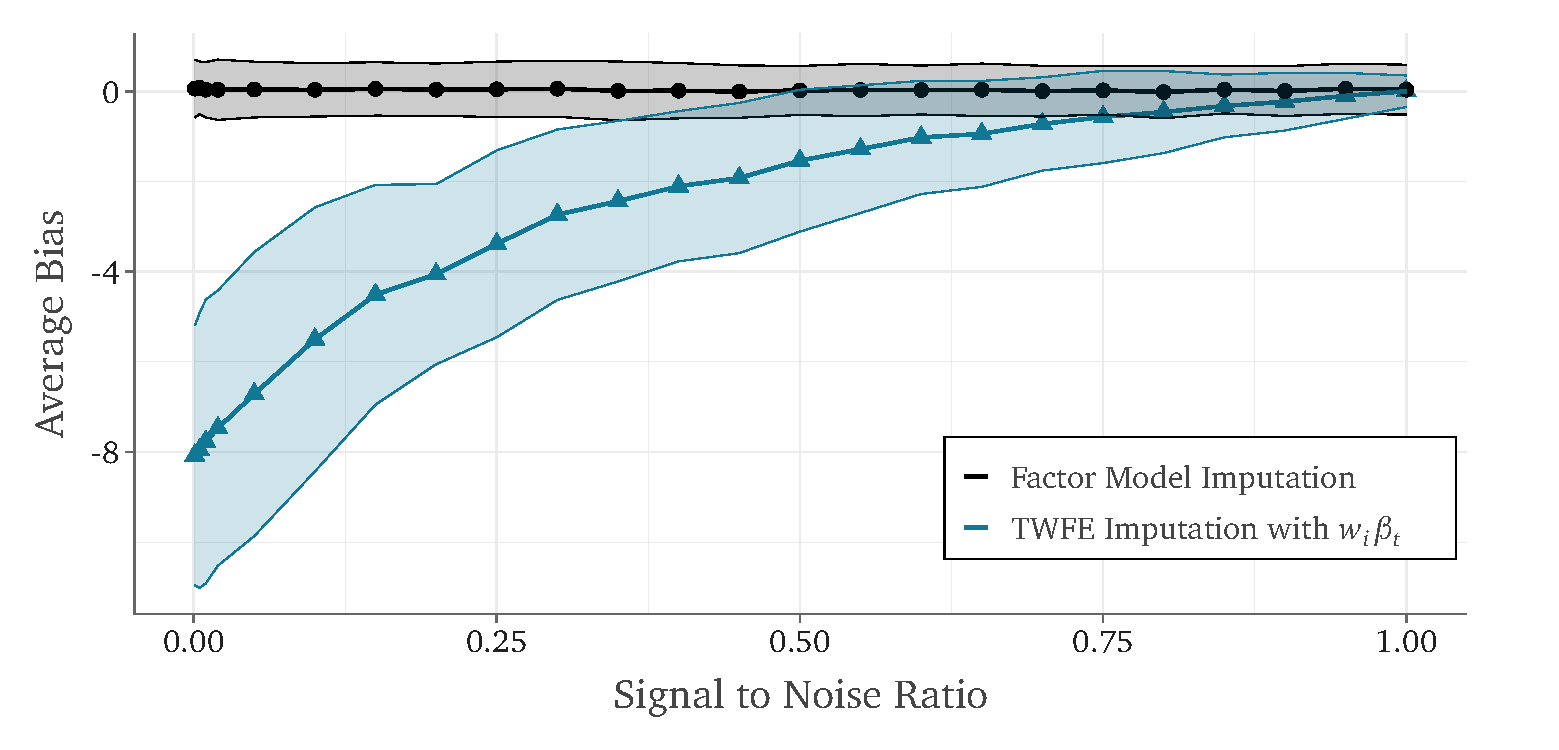
\includegraphics{../figures/simulation-bias_signal_to_noise.pdf}
\end{adjustbox}
\caption{Bias of TWFE Imputation with Covariates}\label{fig:noisy_w}
\note{This figure plots the average and empirical 95\% confidence intervals for treatment effect estimates in the final period, $\hat{\tau}_8$. We estimate the TWFE imputation estimator that includes $w_i \beta_t$ linearly in the model and our the factor imputation we propose using $w_i$ instead as an instrument. We vary the signal to noise ratios of $w_i$ to make it a better or worse measure for the factor loading. For each signal to noise ratio, we run 5000 simulations.}
\end{figure}


% ------------------------------------------------------------------------------
\section{Application}\label{sec:application}
% ------------------------------------------------------------------------------

We revisit the literature on estimating local labor market effects of Walmart store openings \citep{basker2005job, neumark2008effects, volpe2022economic}. The primary identification concern is that Walmart targets where to open stores based on local economic trajectories \citep{neumark2008effects}. For instance, if Walmart targeted areas with positive underlying economic fundamentals in anticipation of their growing consumptive expenditures, then the non-treated counties would fail to be a valid counterfactual group in the two-way error model. Indeed, we observe significant differences in both employment trends for treated counties in our data. \citet{volpe2022economic} point to conflicting results on retail employment with two leading papers finding effects of opposite signs. Employing different instrumental variable strategies, \citet{basker2005job} finds positive effects on retail employment while \citet{neumark2008effects} finds negative effects. For this reason, we revisit this question with an alternative strategy to answer this question. 

We construct a dataset following the description in \citet{basker2005job}. In particular, we use the County Business Patterns dataset from 1964 and 1977-1999, subsetting to counties that (i) had more than 1500 employees overall in 1964 and (ii) had non-negative aggregate employment growth between 1964 and 1977.\footnote{We use the 1977-1999 dataset with imputed values from \citet{eckert2021imputing}.} We use a geocoded dataset of Walmart openings from \citet{arcidiacono2020competitive} to construct our treatment variable. Our treatment dummy is equal to one if the county has any Walmart in that year and our group variable denotes the year of entrance for the \emph{first} Walmart in the county. \footnote{For our sample 82.4\% of our counties receive $\leq 1$ Walmart and another 10.4\% receive two Walmarts in the sample, alleviating some concerns of making the treatment binary.} We drop any county that was treated with $g \leq T_0 = 1985$ so that we we have 9 pre-periods to use when estimating the factor model. Our remaining sample consists of 1274 counties (about 500 fewer than the sample used in \citet{basker2005job} since we drop units treated between 1977 and 1985). We estimate impacts on retail and wholesale employment.\footnote{Retail employment corresponds with NAICS 2-digit codes 44 and 45 and wholesale employment corresponds to NAICS 2-digit code 42.} Walmart is a more vertically integrated business, so we expect Walmart to compete in the retail and the wholesale sectors \citep{basker2005job}.

First, we estimate the two-way fixed effect imputation estimator proposed by \citet{Borusyak_Jaravel_Spiess_2021} and estimate event-study effects on ($\log$) retail and wholesale employment. In particular, we use the following model
\begin{equation}\label{eq:Walmart_twfe}
  \log(y_{it}) = \mu_i + \lambda_t + \sum_{\ell=-22}^{13} \tau^\ell d_{it}^\ell + u_{it}
\end{equation}
where $i$ denotes county, $t$ denotes year, $y_{it}$ is either retail or wholesale employment, and $d_{it}^\ell = 1(t - g_i = \ell)$ are indicator variables denoting event-time. Results of the event-study estimates are presented in panel (a) of figure \ref{fig:walmart_retail} and figure \ref{fig:walmart_wholesale}.

For both retail and wholesale employment, counties receiving Walmarts had faster employment growth relative to the control counties, emphasizing our concern over endogenous opening decisions. In the spirit of \citet{Freyaldenhoven_Hansen_Perez_Shapiro_2022} and \citet{rambachan2023more}, we draw the line of best fit for the 15 most-recent pre-treatment estimates ($\hat{\tau}^\ell$ for $-15 \leq \ell < 0$) and extend it into the post-treatment estimates. For both retail and wholesale employment, the pre-trend lines would suggest that a large portion of the estimated effect is a continuation of already existing trends. However, there still appears to be positive effects on retail employment (if the pre-trend violations were indeed linear in the post-treatment period). 

\begin{figure}
\caption{Effect of Walmart on County $\log$ Retail Employment}
\label{fig:walmart_retail}

\begin{center}
\begin{subfigure}[b]{0.75\textwidth}
  \caption{TWFE Imputation Estimator}
  \begin{adjustbox}{width=\textwidth, center}
    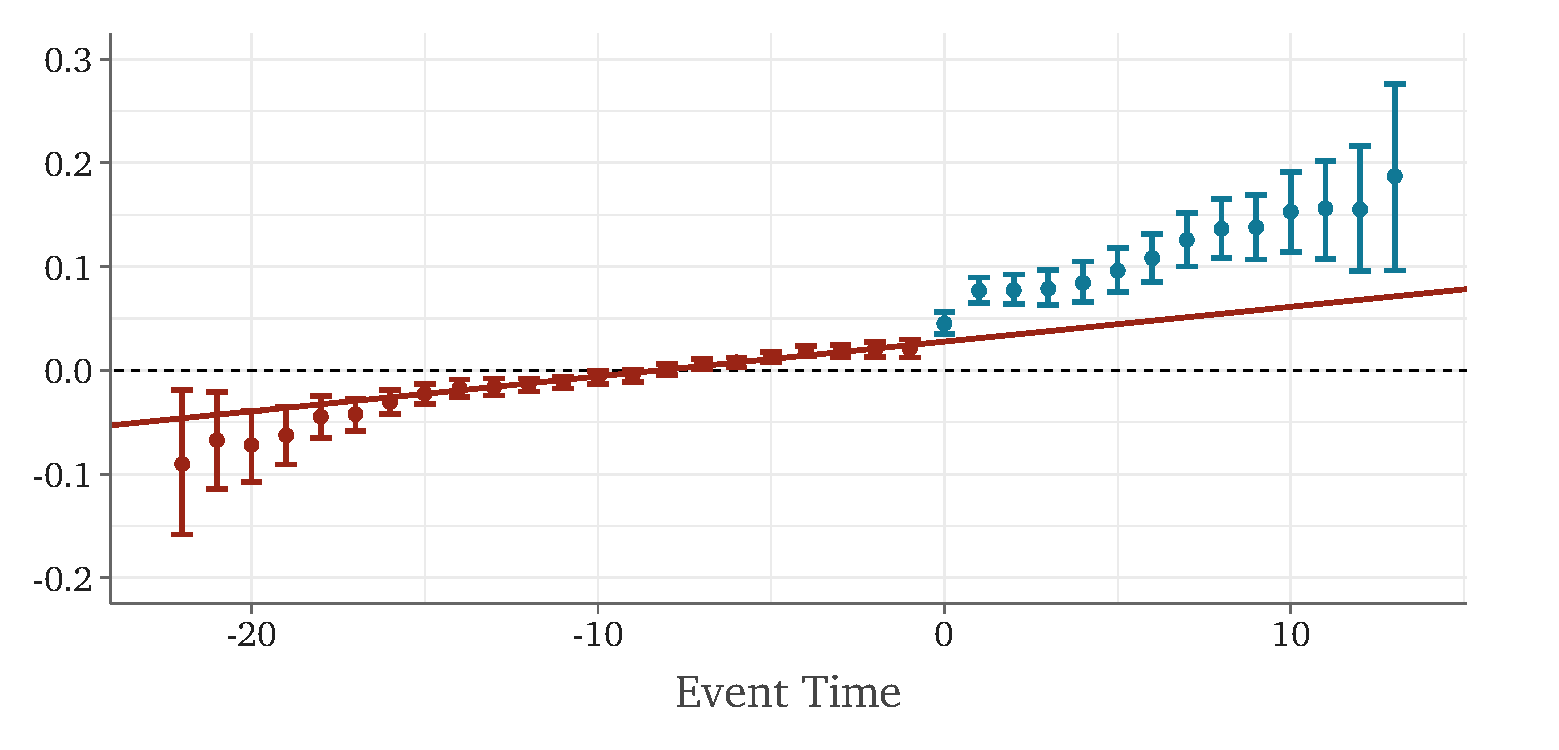
\includegraphics{../figures/plot_did2s_retail.pdf}
  \end{adjustbox}
\end{subfigure}
\end{center}
\begin{center}
\begin{subfigure}[b]{0.75\textwidth}
  \caption{Generalized Imputation Estimator}
  \begin{adjustbox}{width=\textwidth, center}
    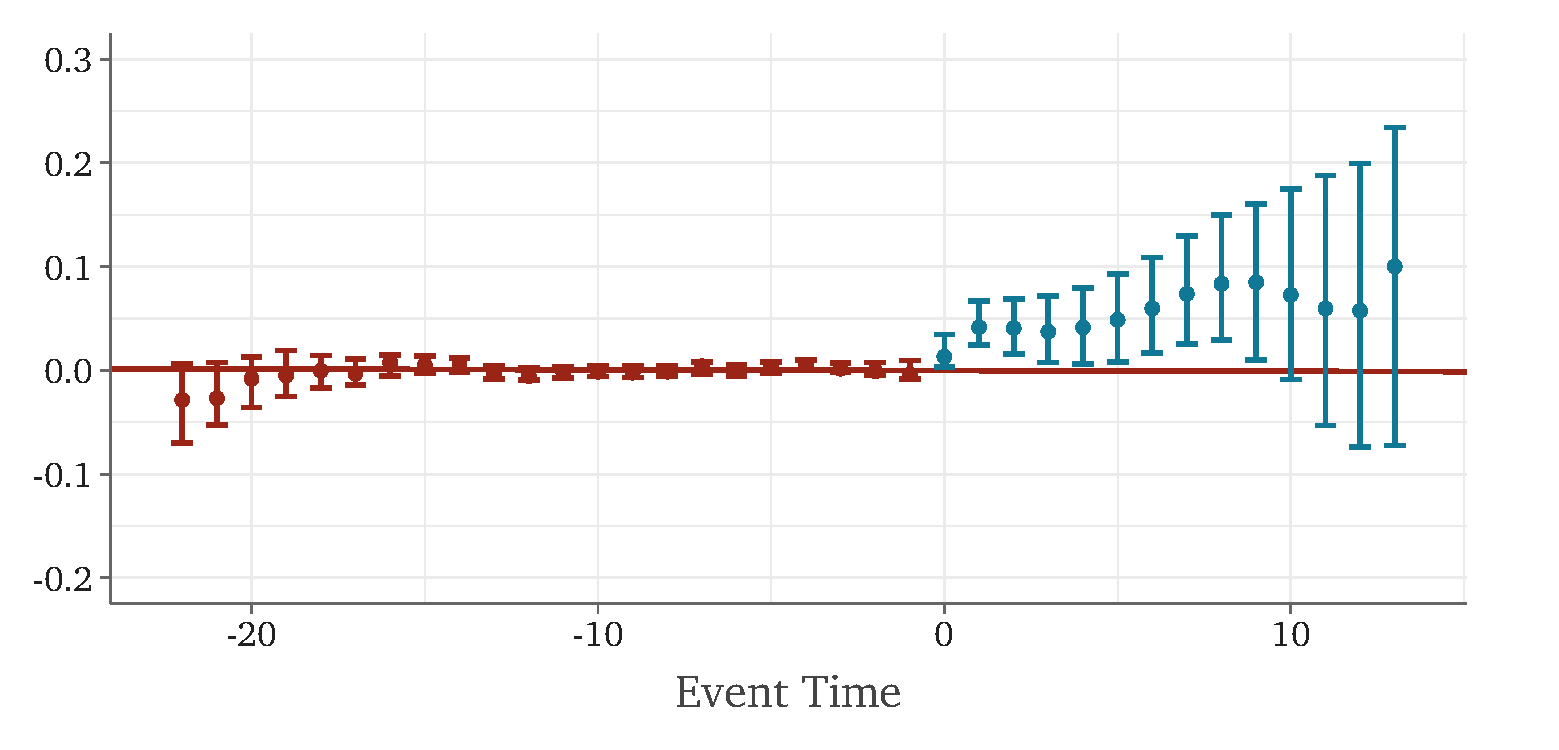
\includegraphics{../figures/plot_qld_retail.pdf}
  \end{adjustbox}
\end{subfigure}
\end{center}

\note{This figure plots point estimates and bootstrapped 95\%  confidence intervals for event-study treatment effects on $\log$ retail employment. Panel (a) estimates effects using the TWFE imputation estimator proposed in \citet{Borusyak_Jaravel_Spiess_2021}. Panel (b) estimates effects using the generalized imputation estimator we propose in Section \ref{sec:estimation} with $p = 2$ and using the following instruments: 1980 share of population employed in manufacturing, 1980 shares of population below and above poverty line; 1980 shares of population employed in private-sector and by the government, 1980 shares of population with high-school degree and college degree. The red lines correspond to a linear estimate of pre-treatment point estimates for event time -15 to -1 and is extended into the post-treatment periods.}
\end{figure}

We use the QLD estimator of \citet{Ahn_Lee_Schmidt_2013} to estimate the factors as described in remark \ref{remark:QLD}. For this factor estimator, we need a set of instruments that satisfy the two standard instrument requirements: relevancy and exclusion. Intuitively, the relevancy restriction requires that the instruments are correlated with the full vector of factor-loadings. That is, the instruments should be selected as `proxies' for the kinds of economic factor-loadings that the researcher is concerned of. The exclusion restriction requires that the instrument values are uncorrelated with location-specific idiosyncratic shocks. For this reason, we use baseline covariate values as instruments to avoid shocks to the covariates that are correlated with shocks to the outcome variable. 

We select instruments that we suspect are driven by the general macroeconomic trends that cause differential retail employment growth in the 1980s and 1990s. For example, retail employment is likely driven by consumptive expenditures which in turn are reflective of local labor market trends. Therefore, we use instruments that we think proxy for characteristics that determine local labor market trends. Specifically, we use the 1980 baseline values of the following variables as instruments: share of population employed in manufacturing, shares of population below and above the poverty line; shares of population employed in the private-sector and by the government, and shares of population with high-school and college degrees.\footnote{All of these values are obtained from 1980 Census Tables accessed from \citet{manson2020ipums}.} We use baseline shares to prevent our instruments from picking up on contemporaneous economic shocks that could be correlated with Walmart opening, i.e. to avoid violations of the exclusion restriction. Note that instead of estimating $\ATT(g,t)$, we estimate $\ATT^\ell$ pooling across $(i, t)$ with $\ell = t - g_i$ as described after Theorem \ref{theorem:asymptotic_distribution}.

\begin{figure}
\caption{Effect of Walmart on County $\log$ wholesale Employment}
\label{fig:walmart_wholesale}

\begin{center}
\begin{subfigure}[b]{0.75\textwidth}
  \caption{TWFE Imputation Estimator}
  \begin{adjustbox}{width=\textwidth, center}
    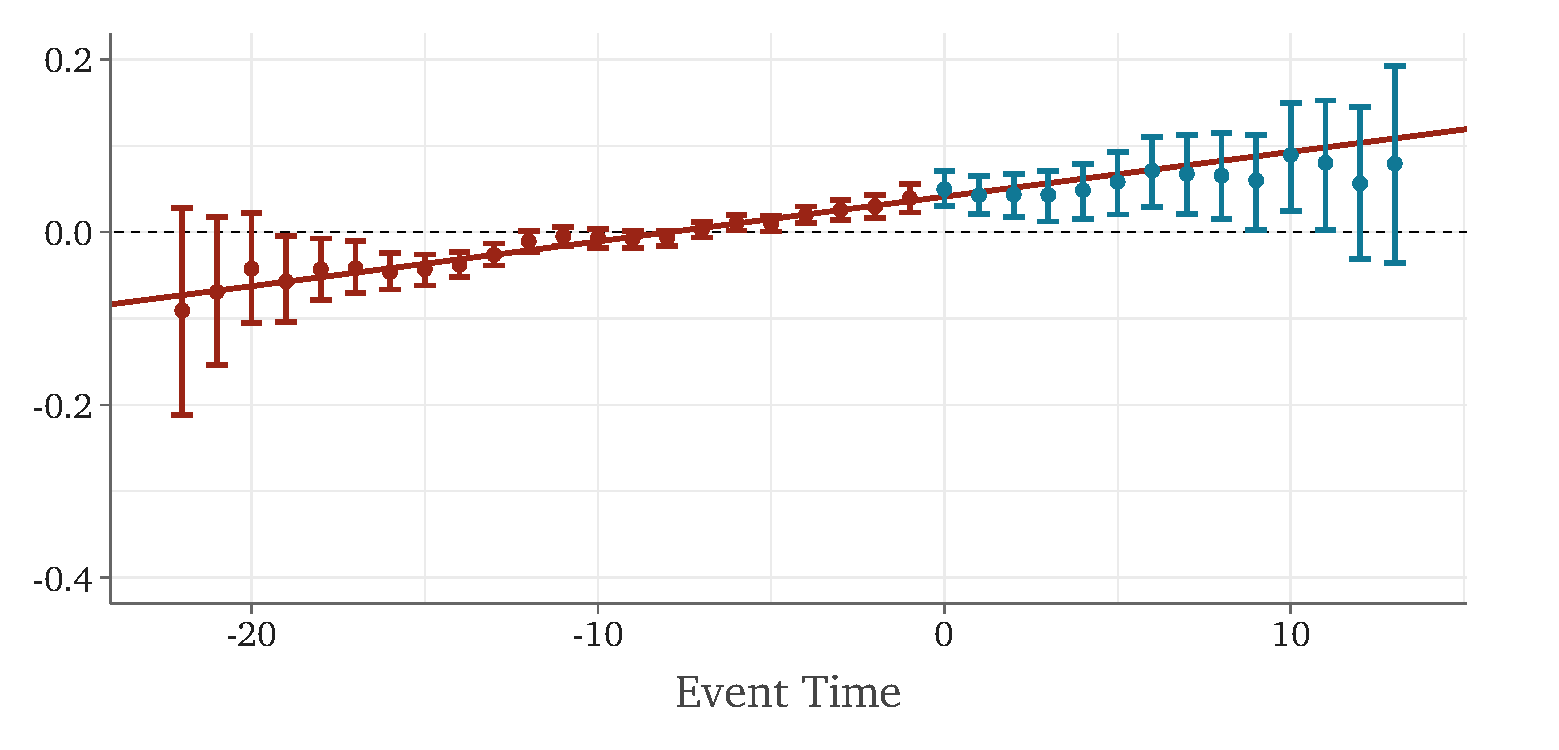
\includegraphics{../figures/plot_did2s_wholesale.pdf}
  \end{adjustbox}
\end{subfigure}
\end{center}
\begin{center}
\begin{subfigure}[b]{0.75\textwidth}
  \caption{Generalized Imputation Estimator}
  \begin{adjustbox}{width=\textwidth, center}
    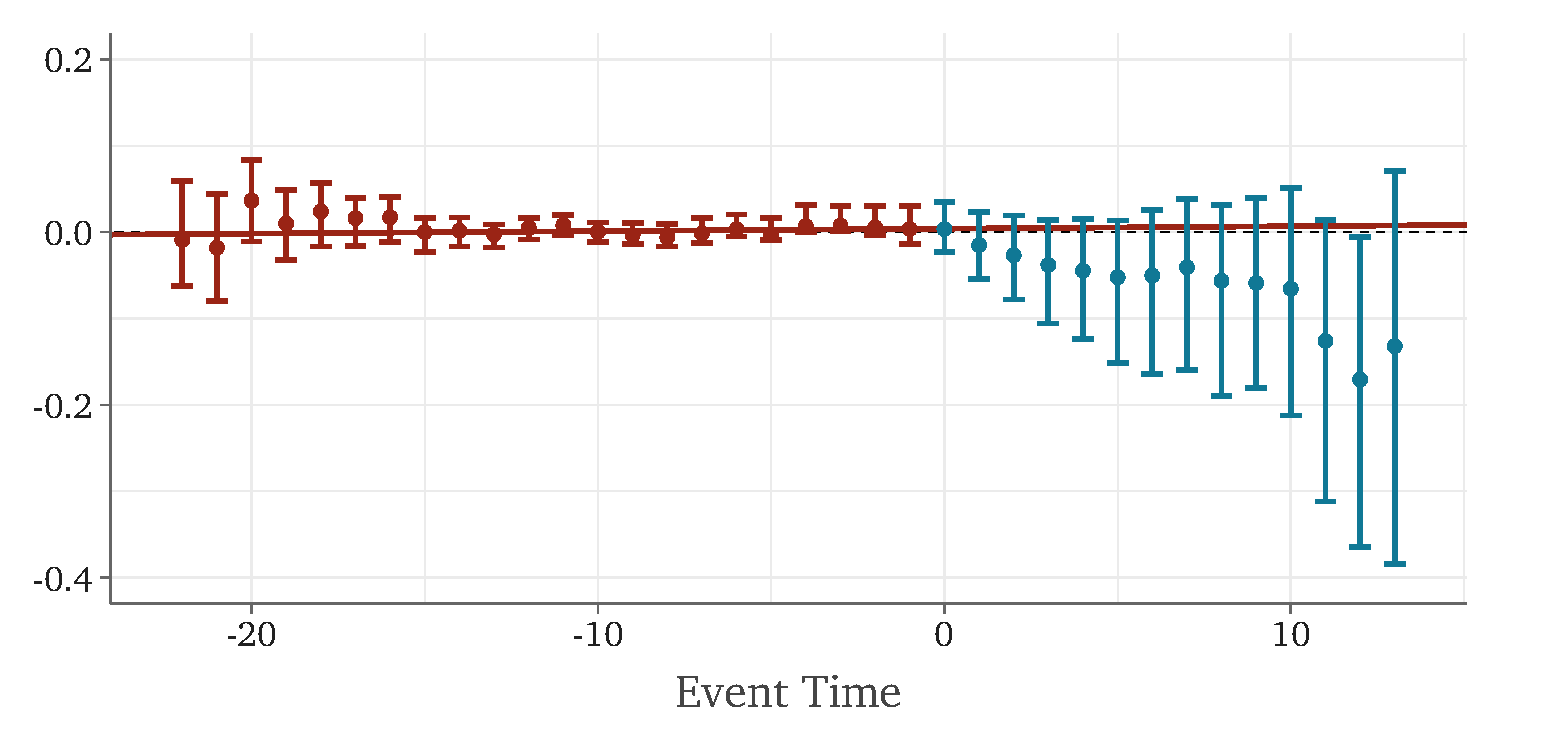
\includegraphics{../figures/plot_qld_wholesale.pdf}
  \end{adjustbox}
\end{subfigure}
\end{center}

\note{This figure plots point estimates and bootstrapped 95\% confidence intervals for event-study treatment effects on $\log$ wholesale employment. Panel (a) estimates effects using the TWFE imputation estimator proposed in \citet{Borusyak_Jaravel_Spiess_2021}. Panel (b) estimates effects using the generalized imputation estimator we propose in Section \ref{sec:estimation} with $p = 1$ and using the following instruments: 1980 share of population employed in manufacturing, 1980 shares of population below and above poverty line; 1980 shares of population employed in private-sector and by the government, 1980 shares of population with high-school degree and college degree. The red lines correspond to a linear estimate of pre-treatment point estimates for event time -15 to -1 and is extended into the post-treatment periods.}
\end{figure}

The results of our estimator are presented in panel (b) of figure \ref{fig:walmart_retail} and figure \ref{fig:walmart_wholesale}.\footnote{We carry out the test to determine the correct number of factors $p$ following the discussion in \citet{Ahn_Lee_Schmidt_2013}. For retail, the p-value of the over-identification test were as follows: p = 0 with a p-value of 1.56e-5; p = 1 with a p-value of 0.001; p = 2 with a p-value of 0.133.  Since $p = 2$ is the first value where we fail to reject the null at a 10\% level, we set $p = 2$. Similarly, we selected $p = 1$ for wholesale since the p-values were: p = 0 with a p-value of 0.049; and p = 1 with a p-value of 0.40.} For retail employment, there is basically no pre-trend violations with the pre-treatment point estimates centered on zero. After removing the pre-existing economic trends, the point estimates are smaller than estimated by the two-way error model with an estimated effect on employment of around 6\% on average in the post-treatment periods. Evaluated at the median baseline retail employment of 1417 employees, this would imply an increase in about 85 jobs, which is in line with the estimates of \citet{basker2005job} and \citet{stapp2014Walmart} who use alternative instrumental variables strategies. It is important to note that post-treatment estimates are noisier than the TWFE estimates largely due to estimating the factor proxies in the first stage. This problem is at its worst for the furthest event-times due to very few counties being averaged over in the last few bins. We view this as a worthy trade-off since the point estimates are much less likely to be biased. 

Turning to wholesale employment, we see a similar story with our estimator removing most of the pre-trend violations. In this case, however, the estimated effects flip signs with an estimated effect of around -6\%, although they are not statistically significant at the 5\% level. Evaluated at the 1977 median wholesale employment of 410, this suggests a decrease of about 25 jobs, which is similar to what \citet{basker2005job} finds. Overall, we find effects very much in line with those reported in \citet{basker2005job}.

Our estimator allows for any root-$N$ consistent estimator of the factor's column space to be `plugged-in' and used for estimation of treatment effects. To show the versatility of the method, we use three different factor estimators in figure \ref{fig:many_factor_estimators}. First, we use our original quasi-differencing estimator from figure \ref{fig:walmart_retail}. Second, we use the common correlated effects (CCE) estimator originally proposed in \citet{pesaran2006estimation}. This estimator uses a set of covariates, $\bm X$, which are generated by the same factors, $\bm{F}$, as the outcome variable:
\begin{equation}
  X_{it} = \bm\alpha_i' \bm{F}_t + \nu_{it}.
\end{equation}
Under this assumption, the cross-sectional averages of $X$ (averaged over the never-treated group) consistently span the column space of $\bm{F}$.  In our application, we use log employment for the manufacturing, construction, agriculture, and healthcare 2-digit NAICS codes. The choice of these covariates is plausible if the same sort of national shocks that affect retail employment also affect these other sectors. We more formally analyze this estimator in \citet{Brown_Butts_Westerlund_2023}, which derives the asymptotic distribution of the estimates. One advantage of this factor estimator is that it allows decomposition of treatment effects into direct effects and mediated effects that operate through the covariates, $X_{it}$.

Last, we use the principal components estimator originally proposed in \citet{Bai_2009}. This estimator uses the eigenvectors  of the matrix $\bm Y \bm Y'$ with the $p$ largest eigenvalues as estimates for $\bm{F}$.\footnote{This imputation estimator is proposed by \citet{Xu_2017} in the context of large panels. The author uses an alternative identification strategy that fails to work in short-panels.} The advantage of this estimator is that no instrument or additional covariates are required. However this comes at the cost of requiring long panels, which may be infeasible to assume in our application.

\begin{figure}
\caption{Generalized Imputation Estimator for Effect of Walmart on County Employment with Different Factor Estimators}
\label{fig:many_factor_estimators}

\begin{center}
\begin{subfigure}[b]{0.75\textwidth}
  \caption{$\log$ Retail Employment}
  \begin{adjustbox}{width=\textwidth, center}
  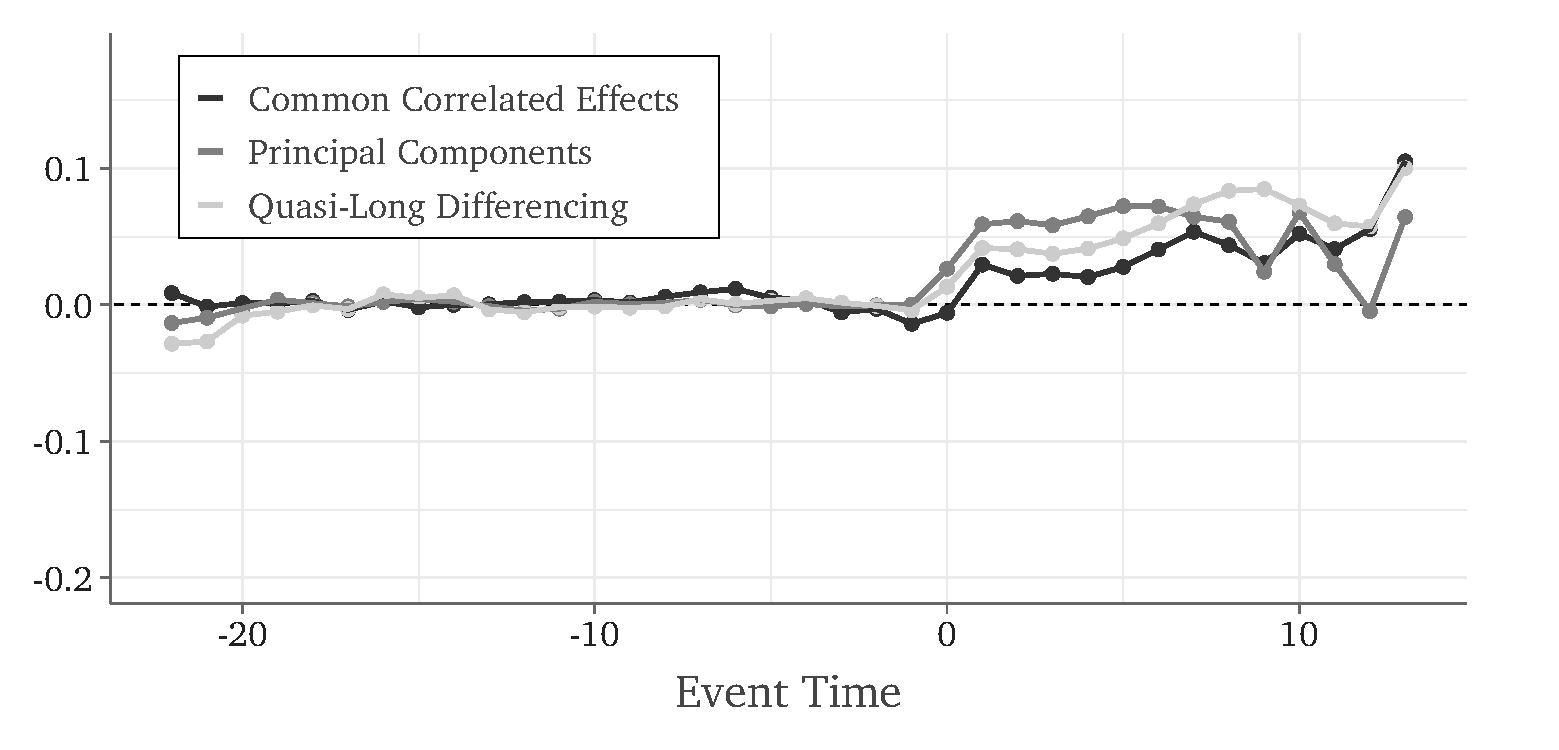
\includegraphics{../figures/plot_retail_many_estimators.pdf}
  \end{adjustbox}
\end{subfigure}
\end{center}
\begin{center}
\begin{subfigure}[b]{0.75\textwidth}
  \caption{$\log$ wholesale Employment}
  \begin{adjustbox}{width=\textwidth, center}
  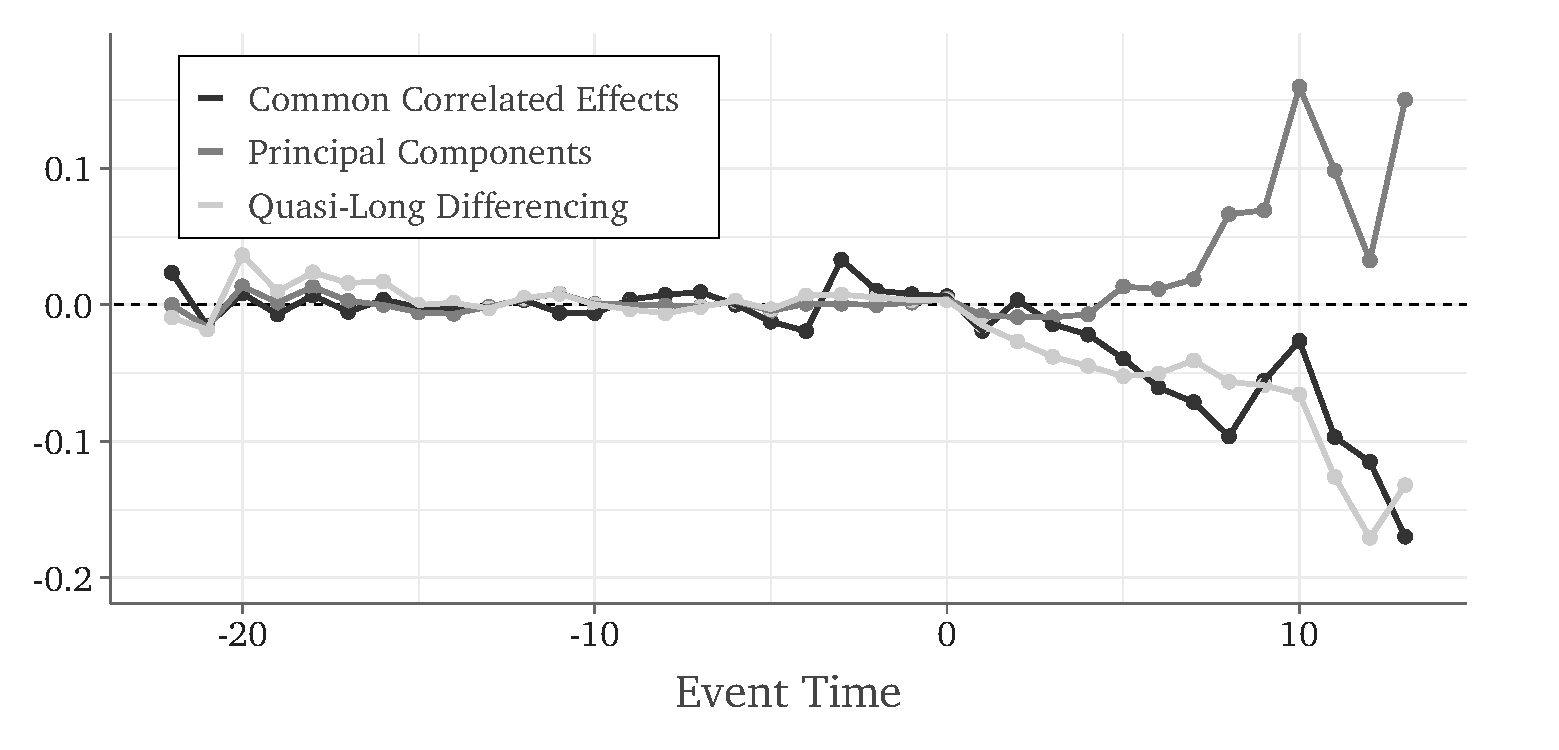
\includegraphics{../figures/plot_wholesale_many_estimators.pdf}
  \end{adjustbox}
\end{subfigure}
\end{center}

\note{This figure presents estimated treatment effects of Walmart entry on county-level $\log$ retail employment using the generalized imputation procedure proposed in section \ref{sec:ATT_identification}. The factor estimation procedures include the principal components estimator proposed in \citet{Bai_2009}, the common correlated effects estimator proposed in \citet{pesaran2006estimation}, and the quasi-differencing estimator proposed in \citet{Ahn_Lee_Schmidt_2013}. Details of the estimation procedures appear in the text.}
\end{figure}

The results of each estimator are presented in figure \ref{fig:many_factor_estimators}. All three estimators are effective at removing underlying trends that the treated counties experienced. Moreover, the estimated effects are similar between estimators suggesting that all three are doing a good job at estimating the underlying factors. This figure highlights the broad applicability of our identification results, allowing the factor estimator of choice to be tailored to the research context at hand. In panel (b), we use $\log$ wholesale employment as an outcome. The CCE and the quasi-differencing estimators produce very similar results, while the principal components estimator suggests positive growth in employment outcomes in later years. Corresponding confidence intervals are very large, suggesting that these results are too noisy to draw any meaningful conclusions. This could be due to wholesale employment being too auto-correlated for the factor estimates to be consistent, or because we do not have a large enough time series to get a meaningful asymptotic approximation of the factors.

% As we discuss above, one reason the synthetic control literature is increasingly popular is that it allows researchers to transparently plot the counterfactual estimates of $y(0)$ for the treated unit. For this reason, we plot the observed $\tilde{y}_{it}$ and the imputed $\hat{\tilde{y}}_{it}(0)$ for (log) retail and wholesale employment in figure \ref{fig:synthetic_control_plot}. In pre-treatment ($\ell < 0$), the imputed estimate, our `synthetic control' follows closely with the observed $\tilde{y}_{it}$ giving us confidence in our ability to approximate the factor structure. In the post-periods, we see the observed counties and the imputed untreated version of the counties pulling apart. The gap between the two are our estimated treatment effects. 
% 
% \begin{figure}
% \caption{Synthetic Control Style Plot of the Effect of Walmart on County Employment}
% \label{fig:synthetic_control_plot}
% 
% \begin{subfigure}[b]{0.49\textwidth}
%   \caption{$\log$ Retail Employment}
%   \begin{adjustbox}{width=\textwidth, center}
%     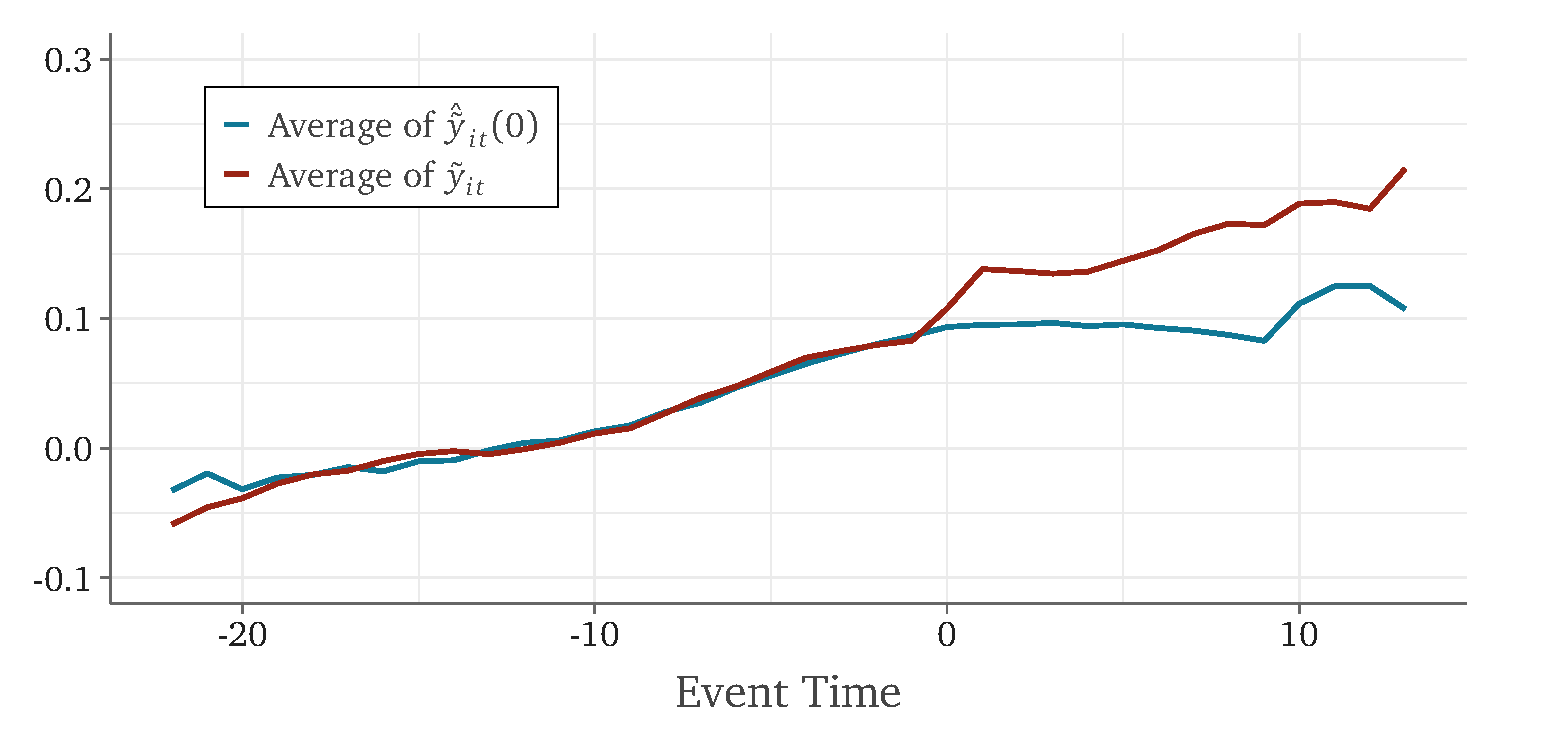
\includegraphics{../figures/plot_synth_retail.pdf}
%   \end{adjustbox}
% \end{subfigure}
% \hfill
% \begin{subfigure}[b]{0.49\textwidth}
%   \caption{$\log$ wholesale Employment}
%   \begin{adjustbox}{width=\textwidth, center}
%     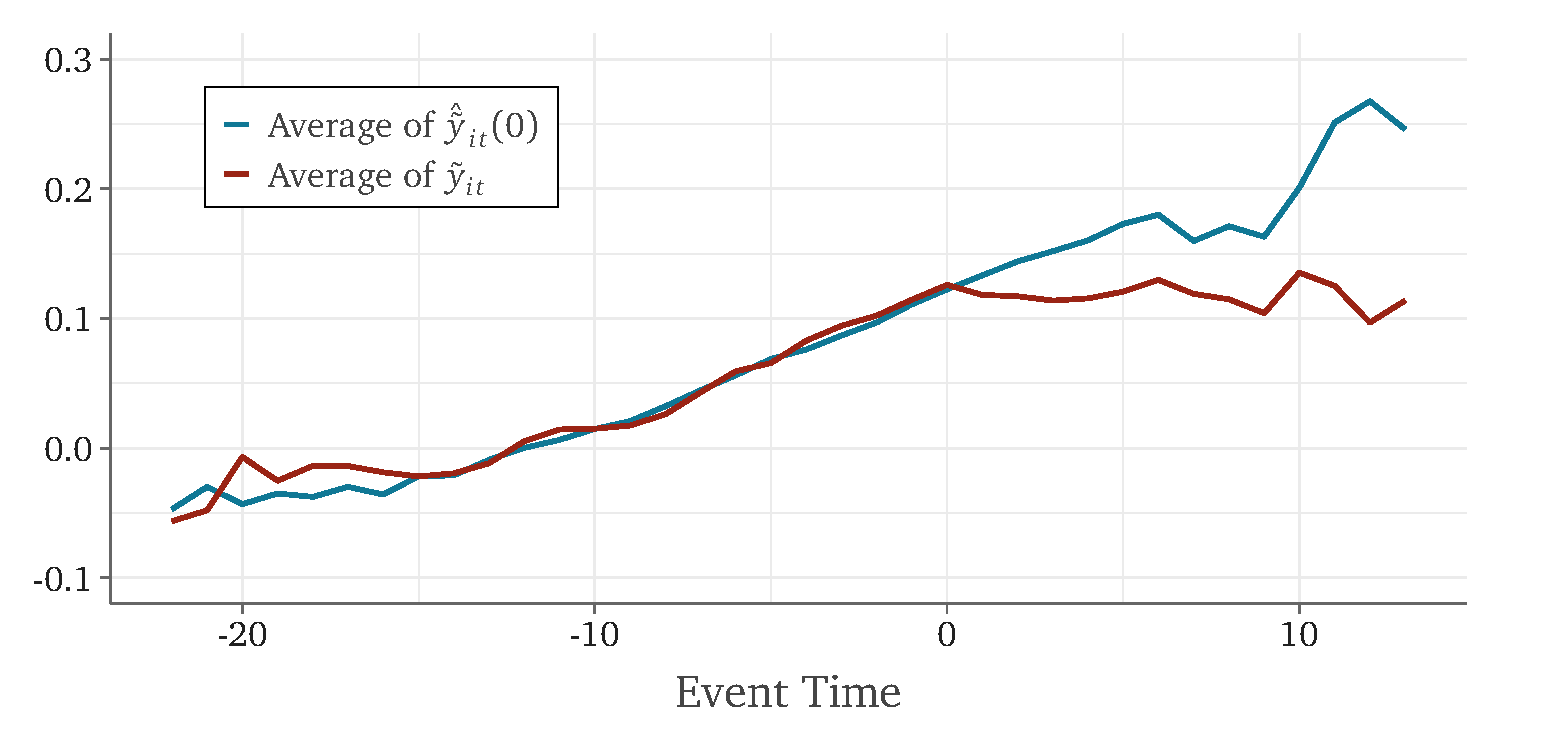
\includegraphics{../figures/plot_synth_wholesale.pdf}
%   \end{adjustbox}
% \end{subfigure}
% 
% \note{This figure plots the observed $\tilde{y}_{it}$ and the imputed $\hat{\tilde{y}}_{it}(0)$ for treated units averaged over event time $\ell = t - g_i$. We impute within-transformed potential outcome using the generalized imputation estimator we propose in Section \ref{sec:estimation} using the following instruments: 1980 share of population employed in manufacturing, 1980 shares of population below and above poverty line; 1980 shares of population employed in private-sector and by the government, 1980 shares of population with high-school degree and college degree.}
% \end{figure}

To highlight the importance of the uncertainty from estimation of the factors in the first stage, we recreate confidence intervals from our generalized imputation estimator with the QLD first stage using the nonparametric standard errors that are derived in Theorem \ref{theorem:nonparametric_variance}. Results are given in figure \ref{fig:Walmart_naive_se}. The standard errors on point estimates are far smaller, with estimates becoming strongly significant in wholesale Employment. This result shows an important step for future research in finding more efficient estimates of the factors. For instance, we consider the common correlated effects estimator in a follow-up paper. The CCE model generally implies that the nonparametric standard errors are valid when there is a common factor model for time-varying covariates.

\begin{figure}
\caption{Generalized Imputation Estimator for Effect of Walmart on County Employment with Naive Standard Errors}
\label{fig:Walmart_naive_se}

\begin{subfigure}[b]{0.49\textwidth}
  \caption{$\log$ Retail Employment}
  \begin{adjustbox}{width=\textwidth, center}
    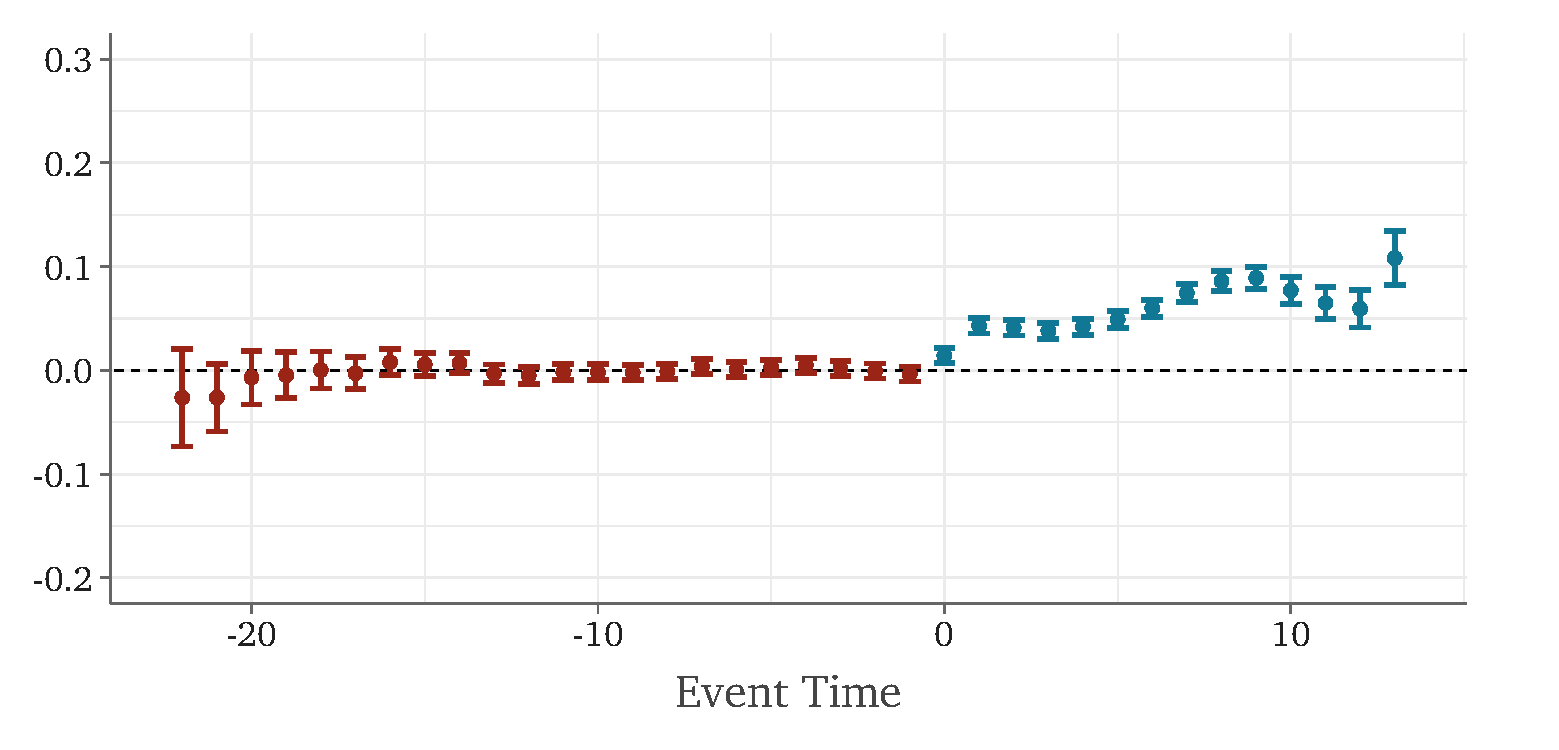
\includegraphics{../figures/plot_qld_retail_naive_se.pdf}
  \end{adjustbox}
\end{subfigure}
\hfill
\begin{subfigure}[b]{0.49\textwidth}
  \caption{$\log$ wholesale Employment}
  \begin{adjustbox}{width=\textwidth, center}
    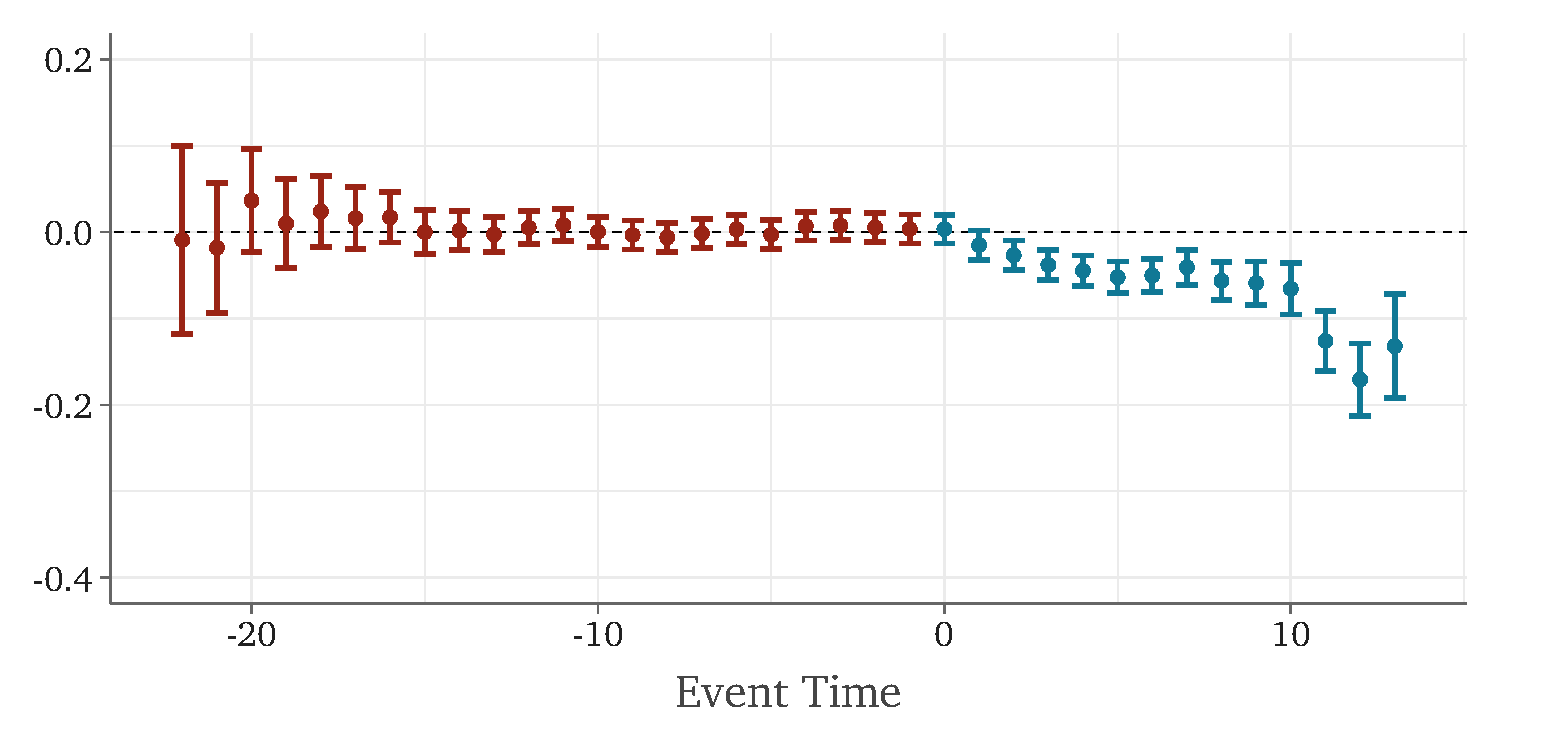
\includegraphics{../figures/plot_qld_wholesale_naive_se.pdf}
  \end{adjustbox}
\end{subfigure}

\note{This figure recreates estimates from panel (b) of figure \ref{fig:walmart_retail} and figure \ref{fig:walmart_wholesale} with confidence intervals formed ignoring the uncertainty deriving from first-stage estimates of $\theta$.}
\end{figure}


% ------------------------------------------------------------------------------
\section{Conclusions}\label{sec:conclusion}
% ------------------------------------------------------------------------------

We consider identification and inference of functions of heterogeneous treatment effects in a linear panel data model. We show how to relax the usual parallel trends assumption by introducing a linear factor model in the error. Our main identification result shows that a consistent estimator of the unobserved factors is all that one needs to estimate the dynamic treatment effect coefficients. This result is general and can be implemented by a number of modern interactive fixed effects estimators, such as quasi-long-differencing, internally generated instruments, common correlated effects, or principal components, allowing for both large and small numbers of pre-treatment time periods. Further work can demonstrate both theoretical and finite-sample properties of these various estimators of the factors and how they affect to ATT estimation, especially for larger time series. The GMM imputation framework should also be examined in the context of unbalanced panels as in \citet{Rai_2022}. 

While a factor model nests the usual two-way error structure, we explicitly model the level fixed effects in addition to the factors. This setting allows us to provide useful tests for the consistency of the TWFE estimator. We also show that one must remove the unit and time fixed effects in a particular way so as to preserve the common factor structure in all time periods for all individuals. We provide such a transformation and prove a novel identification result for TWFE imputation estimators of ATTs.

We implement the QLD estimator of \citet{Ahn_Lee_Schmidt_2013} in a study of the local impact of Walmart openings. We demonstrate findings consistent with the IV estimation strategy of \citet{basker2005job}.  Our estimator is shown to remove pre-trends that bias the usual TWFE estimates. Similar results are found using common correlated effects in the first stage. A principal components estimator is also explored, but performs suspiciously for the given problem. The QLD identification scheme can also allow sequentially exogenous outcomes like those generated by dynamic models. We leave this possibility for future study. 


% \newpage~\section*{Acknowledgements}



% ------------------------------------------------------------------------------
\bibliography{references.bib}
\newpage~\appendix
% ------------------------------------------------------------------------------

\begin{center}
    Appendix for ``\textbf{Dynamic Treatment Effect Estimation with Interactive Fixed Effects and Short Panels}''
\end{center}

% ------------------------------------------------------------------------------
\section{Proofs}\label{sec:proofs}
% ------------------------------------------------------------------------------



\subsection*{Proof of \autoref{theorem:ATT_identification}}

Let $t \geq g$ for the given group $g$.

\begin{equation*}
    \expec{y_{it} - \bm P(\bm{F}_{t}', \bm{F}_{t < g}) \bm y_{i,t < g}}{G_i = g} = \expec{y_{it}(1)}{G_i = g} - \expec{\bm P(\bm{F}_{t}', \bm{F}_{t < g}) \bm y_{i,t < g}}{G_i = g} 
\end{equation*}
We use the fact that 
\begin{align*}
    \expec{ \bm P(\bm{F}_{t}', \bm{F}_{t < g}) \bm y_{i,t < g} }{G_i = g} 
    &= \expec{ \bm{F}_{t}' (\bm{F}_{t < g}' \bm{F}_{t < g})^{-1} \bm{F}_{t < g}' \bm y_{i,t < g} }{G_i = g} \\
    &= \expec{ \bm{F}_{t}' (\bm{F}_{t < g}' \bm{F}_{t < g})^{-1} \bm{F}_{t < g}' \big[\bm{F}_{t < g} \bm \gamma_i + u_{i,t < g} \big] }{G_i = g} \\
    &= \expec{ \bm{F}_{t}' \bm \gamma_i + \bm{F}_{t}' (\bm{F}_{t < g}' \bm{F}_{t < g})^{-1} \bm{F}_{t < g}' u_{i,t < g} }{G_i = g} \\
    &= \expec{ y_{it}(\infty) }{G_i = g} 
\end{align*}
The second equality hold by Assumption 2 and the fact that $y_{i,t < g} = y_{i, t < g}(0)$. The final equality holds by Assumption 2.

For the second part of the theorem, note that from the column span condition, there exists a $m \times p$ matrix $\bm A$ such that 
\begin{equation}
    \bm{F}^*\bm A = \bm{F}
\end{equation}
$\bm A$ defines the linear combinations of the columns of $\bm{F}^*$ that span the columns of $\bm{F}$. Thus $\bm{F}_t^{*'} \bm A = \bm{F}_t'$. We then have
\begin{align*}
    \bm{F}^{*'}_t (\bm{F}^{*'}_{t < g} \bm{F}^{*'}_{t < g})^{-1} \bm{F}^{*'}_{t < g} \bm{F}_{t < g} \bm \gamma_i
    &= \bm{F}^{*'}_t (\bm{F}^{*'}_{t < g} \bm{F}^{*}_{t < g})^{-1} \bm{F}^{*'}_{t < g} \bm{F}^{*'}_{t < g} \bm A \bm \gamma_i \\
    &= \bm{F}^{*'}_t \bm A \bm \gamma_i \\
    &= \bm{F}^{*'}_t \bm \gamma_i
\end{align*}

If $m = p$ so that $\bm{F}$ also has full column rank, we can make the stronger statement that the imputation matrices of $\bm{F}$ and $\bm{F}^{*}$ are equal: 
    \begin{align*}
        \bm P (\bm{F}_{t \geq g}, \bm{F}_{t < g}) 
        &= \bm{F}_{t \geq g} (\bm{F}_{t < g}' \bm{F}_{t < g})^{-1} \bm{F}_{t < g}' \\
        &= \bm{F}_{t \geq g} \bm A (\bm A'\bm{F}_{t < g}' \bm{F}_{t < g} \bm A)^{-1} \bm A' \bm{F}_{t < g}' \\
        &= \bm{F}^{*'}_{t \geq g} (\bm{F}^{*'}_{t < g} \bm{F}^{*}_{t < g})^{-1} \bm{F}^{*'}_{t < g} \\
        &= \bm P(\bm{F}^{*}_{t \geq g}, \bm{F}^{*}_{t < g})
    \end{align*}
    where the second equality holds because $\bm A$ and $(\bm{F}_{t < g}' \bm{F}_{t < g})$ are full rank.

$\square$

\subsection*{Proof of Lemma 2.1}

We first derive the averages defined in Section 2.2 in terms of the potential outcome framework:
\begin{gather*}
    \overline{y}_{\infty , t} = \frac{1}{N_{\infty}} \sum_{i = 1}^N D_{i \infty} y_{it} = \overline{\mu}_{\infty} + \lambda_t + \bm{F}_t \overline{\bm \gamma}_{\infty} + \overline{u}_{t, \infty}\\
    \overline{y}_{i,t\leq T_0} = \frac{1}{T_0} \sum_{t = 1}^{T_0} y_{it} = \mu_i + \overline{\lambda}_{t < T_0} + \overline{\bm{F}}_{t < T_0} \bm \gamma_i + \overline{u}_{i,t < T_0}\\
    \overline{y}_{\infty, t < T_0} = \frac{1}{N_{\infty} T_0} \sum_{i = 1}^N \sum_{t = 1}^{T_0} D_{i \infty} y_{it} = \overline{\mu}_{\infty} + \overline{\lambda}_{t < T_0} + \overline{\bm{F}}_{t < T_0} \overline{\bm \gamma}_{\infty} + \overline{u}_{\infty, t < T_0}
\end{gather*}
where $\overline{\mu}_{\infty}$ and $\overline{\bm \gamma}_{\infty}$ are the averages of the never-treated individuals' heterogeneity and $\overline{\bm{F}}_{t < T_0}$ and $\overline{\lambda}_{t < T_0}$ are the averages of the time effects before anyone is treated. The error averages have the same interpretation as the outcome averages.

The definition of $\tau_{it}$ is the difference between treated and untreated potential outcomes for unit $i$ at time $t$, so for any $(i,t)$, $y_{it} = d_{it} y_{it}(1) + (1-d_{it})y_{it}(\infty) = d_{it} \tau_{it} + y_{it}(\infty)$. Then
\begin{align*}
    \tilde{y}_{it} 
    &= d_{it} \tau_{it} + \bm{F}_t' \bm \gamma_i - \overline{\bm{F}}'_{t < T_0} \bm \gamma_i - \bm{F}_t' \overline{\bm \gamma}_{\infty} + \overline{\bm{F}}_{t < T_0} \overline{\bm \gamma}_{\infty} + u_{it} - \overline{u}_{t,\infty} - \overline{u}_{i, t < T_0} + \overline{u}_{\infty, t < T_0}\\
    &= d_{it} \tau_{it} + (\bm{F}_t - \overline{\bm{F}}_{t < T_0})' (\bm \gamma_i - \overline{\bm \gamma}_{\infty}) + u_{it} - \overline{u}_{t,\infty} - \overline{u}_{i, t < T_0} + \overline{u}_{\infty, t < T_0}
\end{align*}
Taking expectation conditional on $G_i = g$ gives $\expec{u_{it} - \overline{u}_{i, t < T_0}}{G_i = g} = 0$ by Assumption 2 and $\expec{\overline{u}_{\infty, t < T_0} - \overline{u}_{t, \infty} }{G_i = g} = \expec{\overline{u}_{\infty, t < T_0} - \overline{u}_{t, \infty}} = 0$ by random sampling and iterated expectations.

$\square$

\subsection*{Proof of Theorem 3.1}

Asymptotic normality is a consequence of well-known large sample GMM theory. See, for example, \citet{Hansen_1982}.

We only need to derive the asymptotic variances. Note that $\bm g_{i\infty}(\bm{\theta}) \otimes \bm g_{ig}(\bm{\theta}, \bm \tau_g) = \bm 0$ (from the $D_{ig}$ terms) and $\bm g_{ih}(\bm{\theta}, \bm \tau_h) \otimes \bm g_{ik}(\bm{\theta}, \bm \tau_k) = \bm 0$ almost surely uniformly over the parameter space for all $g \in \mathcal{G}$ and $h \neq k$. The covariance matrix of these moment functions, which we denote as $\bm \Delta$, is a block diagonal matrix.
\begin{equation*}
    \bm \Delta =
    \begin{pmatrix}
        \expec{\bm g_{i \infty}(\bm{\theta}) \bm g_{i \infty}(\bm{\theta})'} & \bm 0 & \bm 0 & \hdots & \bm 0\\
        \bm 0 &  \expec{\bm g_{i g_G}(\bm{\theta}, \bm \tau_{g_G}) \bm g_{i g_G}(\bm{\theta}, \bm \tau_{g_G})' } & \bm 0 & \hdots & \bm 0\\
        \vdots & & \ddots  &\\
        \bm 0 & \bm 0 & \bm 0 & \hdots & \expec{ \bm g_{i g_1}(\bm{\theta}, \bm \tau_{g_1}) \bm g_{i g_1}(\bm{\theta}, \bm \tau)'}
    \end{pmatrix}
\end{equation*}
We write the individual blocks as $\bm \Delta_g$ for $g \in \mathcal{G} \cup \{ \infty \}$. The gradient is also simple to compute because all of the moments are linear in the treatment effects. We define the overall gradient $\bm D$ and show it is a lower triangular matrix which we write in terms of its constituent blocks:
\begin{equation*}
    \bm D = 
    \begin{pmatrix}
        \expec{\nabla_{\bm{\theta}} \bm g_{i\infty}(\bm{\theta}) } & \bm 0 & \bm 0 & \hdots & \bm 0\\
        \expec{\nabla_{\bm{\theta}} \bm g_{ig_G}(\bm{\theta}, \bm \tau_{g_G})} & -\bm I_{T - g_G + 1} & \bm 0 & \hdots & \bm 0\\
        \vdots & & \ddots  &\\
        \expec{\nabla_{\bm{\theta}} \bm g_{ig_1}(\bm{\theta}, \bm \tau_{g_1})} & \bm 0 & \bm 0 & \hdots & -\bm I_{T - g_1 + 1}
    \end{pmatrix}
\end{equation*}
where we write the blocks in the first column as $\bm D_g$ for $g \in \mathcal{G} \cup \{ \infty \}$. The diagonal is made up of negative identity matrices because $\expec{\frac{D_{ig_h}}{\mathbb{P}(D_{ig_h} = 1)}} = 1$.

Given we use the optimal weight matrix, the overall asymptotic variance is given by $(\bm D' \bm \Delta^{-1} \bm D)^{-1}$. $\Delta$ is a block diagonal matrix so its inverse is trivial to compute. First, we have
\begin{equation*}
    \bm \Delta^{-1} \bm D = 
    \begin{pmatrix}
        \bm \Delta_{\infty}^{-1} \bm D_{\infty} & \bm 0 &  \hdots & \bm 0\\
        \bm \Delta_{g_G}^{-1} \bm D_{g_G} & -\bm \Delta_{g_G}^{-1} & \hdots & \bm 0\\
        \vdots & & \ddots &\\
        \bm \Delta_{g_1}^{-1} \bm D_{g_1} & \bm 0 & \hdots & - \bm \Delta_{g_1}^{-1}
    \end{pmatrix}
\end{equation*}
The transpose of the gradient matrix is
\begin{equation*}
    \bm D' =
    \begin{pmatrix}
        \bm D_{\infty}' & \bm D_{g_G}' & \hdots & \bm D_{g_1}'\\
        \bm 0 & -\bm I_{T-g_G + 1} & \hdots & \bm 0\\
        \vdots & & \ddots & \\
        \bm 0 & \bm 0 & \hdots & - \bm I_{T-g_1 + 1}
    \end{pmatrix}
\end{equation*}
so that we get
\begin{equation*}
    \bm D' \bm \Delta^{-1} \bm D = 
    \begin{pmatrix}
        \sum_{g \in \mathcal{G}\cup\{\infty\}} \bm D_g' \bm \Delta_g^{-1} \bm D_g & -\bm D_{g_G}' \bm \Delta_{g_G}^{-1} & \hdots & - \bm D_{g_1}' \bm \Delta_{g_G}^{-1}\\
        -\bm \Delta_{g_G}^{-1} \bm D_{g_G} & \bm \Delta_{g_G}^{-1} & \hdots & \bm 0\\
        \vdots & & \ddots &\\
        -\bm \Delta_{g_1}^{-1} \bm D_{g_1} & \bm 0 & \hdots & \bm \Delta_{g_1}^{-1}
    \end{pmatrix}
\end{equation*}

We write this matrix as 
\begin{equation*}
    \begin{pmatrix}
        \bm A & \bm B\\
        \bm C & \bm D
    \end{pmatrix}
\end{equation*}
where $\bm A = \sum_{g \in \mathcal{G}\cup \{\infty\}} \bm D_g' \bm \Delta_g^{-1} \bm D_g$ and $\bm D = \text{diag} \{ \bm \Delta_g^{-1} \}_{g \in \mathcal{G}}$. We then apply Exercise 5.16 of \citet{abadir2005matrix} to get the final inverse. The top left corner of the inverse is $\bm{F}^{-1}$ where
\begin{align*}
    (\bm{F})^{-1} 
    &= (\bm A - \bm B \bm D^{-1} \bm C)^{-1}\\
    &= \left( \sum_{g \in \mathcal{G}\cup\{\infty\}} \bm D_g' \bm \Delta_g^{-1} \bm D_g - \left( \sum_{g \in \mathcal{G}} \bm D_g' \bm \Delta_g^{-1} \bm D_g \right) \right)^{-1}\\
    &= (\bm D_{\infty}' \bm \Delta_{\infty}^{-1} \bm D_{\infty})^{-1}\\
    &= \text{Avar}(\sqrt{N}(\widehat{\bm{\theta}} - \bm{\theta}))
\end{align*}
The rest of the first column of matrices takes the form
\begin{align*}
    -\bm D^{-1} \bm C \bm{F}^{-1}
    &=
    \begin{pmatrix}
        \bm D_{g_G}\\
        \vdots\\
        \bm D_{g_1}
    \end{pmatrix}
    (\bm D_{\infty}' \bm \Delta_{\infty}^{-1} \bm D_{\infty})^{-1}\\
    &=
    \begin{pmatrix}
        \bm D_{g_G} (\bm D_{\infty}' \bm \Delta_{\infty}^{-1} \bm D_{\infty})^{-1}\\
        \vdots\\
        \bm D_{g_1} (\bm D_{\infty}' \bm \Delta_{\infty}^{-1} \bm D_{\infty})^{-1}
    \end{pmatrix}
\end{align*}
and the rest of the first row is $- \bm{F}^{-1} \bm B \bm D^{-1} = (- \bm D^{-1} \bm B' \bm{F}^{-1})' = (- \bm D^{-1} \bm C \bm{F}^{-1})'$.

Finally, the bottom-right block, which also gives the asymptotic covariance matrix of the ATT estimators, is 
\begin{align*}
    \bm D^{-1} + \bm D^{-1} \bm C \bm{F}^{-1} \bm B \bm D^{-1} 
    &= \bm D^{-1} + 
    \begin{pmatrix}
        \bm D_{g_G} (\bm D_{\infty}' \bm \Delta_{\infty}^{-1} \bm D_{\infty})^{-1} \bm D_{g_G}' & \hdots & \bm D_{g_G} (\bm D_{\infty}' \bm \Delta_{\infty}^{-1} \bm D_{\infty})^{-1} \bm D_{g_1}'\\
        & \ddots &\\
        \bm D_{g_1} (\bm D_{\infty}' \bm \Delta_{\infty}^{-1} \bm D_{\infty})^{-1} \bm D_{g_G}' & \hdots & \bm D_{g_1} (\bm D_{\infty}' \bm \Delta_{\infty}^{-1} \bm D_{\infty})^{-1} \bm D_{g_1}'
    \end{pmatrix}
\end{align*}
The $g$'th diagonal elements of the resulting matrix is $\bm \Delta_g + \bm D_g (\bm D_{\infty}' \bm \Delta_{\infty}^{-1} \bm D_{\infty})^{-1} \bm D_g'$.

$\square$




\subsection*{Proof of Theorem 3.2}

We derive the limiting theory by multiplying $\widehat{\bm \Delta}_g$ by $(N_g-1)/N_g$ which produces the same limit as $N \rightarrow \infty$. We write
\begin{equation*}
    \frac{N_g - 1}{ N_g} \widehat{\bm \Delta}_g = \frac{1}{N_g} \sum_{i = 1}^N D_{ig} \widehat{\bm \Delta}_{ig} \widehat{\bm \Delta}_{ig}' - \widehat{\bm \tau}_g \widehat{\bm \tau}_g'
\end{equation*}
We already know that $\widehat{\bm \tau}_g \plim \bm \tau_g$ by Theorem 3.1. Note that 
\begin{align*}
    \frac{1}{N_g} \sum_{i = 1}^N D_{ig} \widehat{\bm \Delta}_{ig} \widehat{\bm \Delta}_{ig}' = &\left( \frac{1}{N_g} \sum_{i = 1}^N D_{ig}  \bm y_{i, t \geq g} \bm y_{i, t \geq g}' \right) - \left( \frac{1}{N_g} \sum_{i = 1}^N D_{ig} \bm y_{i, t \geq g} \bm y_{i, t < g}' \right) \bm P(\bm{F}_{t \geq g}(\widehat{\bm{\theta}}), \bm{F}_{t < g}(\widehat{\bm{\theta}}))'\\
    &- \bm P(\bm{F}_{t \geq g}(\widehat{\bm{\theta}}), \bm{F}_{t < g}(\widehat{\bm{\theta}})) \left( \frac{1}{N_g} \sum_{i = 1}^N D_{ig} \bm y_{i, t < g} \bm y_{i, t \geq g}' \right)\\
    &- \bm P(\bm{F}_{t \geq g}(\widehat{\bm{\theta}}), \bm{F}_{t < g}(\widehat{\bm{\theta}})) \left( \frac{1}{N_g} \sum_{i = 1}^N D_{ig}  \bm y_{i, t < g} \bm y_{i, t \geq g}' \right) \bm P(\bm{F}_{t \geq g}(\widehat{\bm{\theta}}), \bm{F}_{t < g}(\widehat{\bm{\theta}}))'
\end{align*} 

Given $\bm P(\bm{F}_{t \geq g}(\widehat{\bm{\theta}}), \bm{F}_{t < g}(\widehat{\bm{\theta}}))$ is equal to its infeasible counterpart $\bm P(\bm{F}_{t \geq g}, \bm{F}_{t < g})$ plus a $O_p(N^{-1/2})$ term, Assumption 1 and the weak law of large numbers imply 
\begin{equation*}
    \frac{1}{N_g} \sum_{i = 1}^N D_{ig} \widehat{\bm \Delta}_{ig} \widehat{\bm \Delta}_{ig}' - \widehat{\bm \tau}_g \widehat{\bm \tau}_g' \plim \expec{\bm g_{ig}(\bm{\theta}, \bm \tau_g)}{G_i = g} = \bm \Delta_g
\end{equation*}
The inverse exists with probability approaching one by Assumption 5.

$\square$


% ------------------------------------------------------------------------------
\section{Inference of Aggregate Treatment Effects}
% ------------------------------------------------------------------------------

As in \citet{Callaway_Santanna_2021}, we can form aggregates of our group-time average treatment effects. For example, event-study type coefficients would average over the $\tau_{gt}$ where $t - g = e$ for some relative event-time $e$ with weights proportional to group membership. Consider a general aggregate estimand $\delta$ which we define as a weighted average of $ATT(g,t)$:
\begin{equation}
\delta = \sum_{g\in \mathcal{G}} \sum_{t > T_0} w(g,t) \tau_{gt}
\end{equation}
where the weights $w(g,t)$ are non-negative and sum to one. Table 1 of \citet{Callaway_Santanna_2021} and the surrounding discussion describes various treatment effect aggregates and discuss explicit forms for the weights. 

Our plug-in estimate for $\delta$ is given by $\hat{\delta} = \sum_{g\in \mathcal{G}} \sum_{t > T_0} \hat{w}(g,t) \hat{\tau}_{gt}$. Inference on this term follows directly from Corollary 2 in \citet{Callaway_Santanna_2021} if we have the influence function for our $\tau_{gt}$ estimates. Rewriting our moment equations in an asymptotically linear form, we have:
\begin{equation}
    \sqrt{N}\Big( (\widehat{\bm{\theta}}', \widehat{\bm \tau}')' - (\bm{\theta}', \bm \tau')' \Big) = - \left( \frac{1}{\sqrt{N}} \sum_{i = 1}^N (\bm D' \bm \Delta^{-1} \bm D)^{-1} \bm D' \bm \Delta^{-1} \bm g_i(\bm{\theta}, \bm \tau) \right) + o_p(1).
\end{equation}
This form comes from the fact that the weight matrix is positive definite with probability approaching one\footnote{This is a well-known expansion for analyzing the asymptotic properties of GMM estimators. See Chapter 14 of \citet{Wooldridge_2010} for example.}. The first term on the right-hand side is the influence function and hence inference on aggregate quantities follows directly. This result allows for use of the multiplier bootstrap to estimate standard errors in a computationally efficient manner.

% ------------------------------------------------------------------------------
\section{Inference in Two-Way Fixed Effect Model}\label{sec:twfe_inference}
% ------------------------------------------------------------------------------

We derive the asymptotic distribution of our imputation estimator based off of the two-way error model in equation (1). First, we note that this estimator can be written in terms of the imputation matrix from Section 2. In particular, let $\bm 1_t$ be a $T \times 1$ vector of ones up the $t$'th spot, with all zeros after. Define $\overline{\bm y}_{\infty} = (\overline{y}_{\infty, 1},..., \overline{y}_{\infty, T})'$ be the full vector of never-treated cross-sectional averages. Then our imputation transformation can be written as 
\begin{equation}
    \tilde{\bm y}_i = \left[ \bm I_T - \bm P(\bm 1_T, \bm 1_{T_0}) \right] (\bm y_i - \overline{\bm y}_{\infty})
\end{equation}
where the $t^{th}$ component of the above $T$-vector is 
\begin{equation}
    d_{it} \tau_{it} + \tilde{u}_{it},
\end{equation}
with $\tilde{u}_{it}$ is defined as the same transformation as $\tilde{y}_{it}$.

The imputation step of our estimator is a just-identified system of equations. As such, we do not need to worry about weighting in implementation and inference comes from standard theory of M-estimators. In fact, we have the following closed-form solution for the estimator of a group-time average treatment effect: 
\begin{equation}
    \widehat{\tau}_{gt} = \frac{1}{N_{g}}\sum_{i} D_{ig} \tilde{y}_{it},
\end{equation}
where $N_{gt} = \sum_i D_{ig}$ is the number of units in group $g$. 

The following theorem characterizes estimation under the two-way error model:
\begin{theorem}\label{theorem:twfe}
    Assume untreated potential outcomes take the form of the two-way error model given in equation (1). Suppose Assumptions 1 and 3 hold, as well as Assumption 2 with $\bm \gamma_i = 0$. Then for all $(g, t)$ with $g > t$, $\widehat{\bm \tau}_{gt}$ is conditionally unbiased for $\expec{\tau_{it}}{D_{ig} = 1}$, has the linear form
    \begin{equation}\label{eq:twfe_influence}
        \sqrt{N_{g}} \big( \widehat{\tau}_{gt} - \tau_{gt} \big) 
        = \frac{1}{\sqrt{N_{g}}}\sum_{i=1}^N D_{ig} (\tau_{it} - \tau_{gt} + u_{it} - \overline{u}_{i,t < T_0} - \overline{u}_{\infty,t} + \overline{u}_{\infty,t < T_0})
    \end{equation}
    and  
    \begin{equation}\label{eq:twfe_asymptotic}
        \sqrt{N_1}(\widehat{\tau}_{gt} - \tau_{gt}) \convd N(0, V_1 + V_0)
    \end{equation}
    as $N \rightarrow \infty$, where $V_1$ and $V_0$ are given below and $\tau_{gt} = \expec{y_{it}(g) - y_{it}(\infty)}{D_{ig} = 1}$ is the group-time average treatment effect (on the treated). $\blacksquare$
\end{theorem}
Theorem (\ref{theorem:twfe}) demonstrates the simplicity of our imputation procedure under the two-way error model. While the general factor structure requires more care, estimation and inference will yield a similar result.


\subsection*{Proof of Theorem \ref{theorem:twfe}}

The transformed post-treatment observations are
\begin{equation}
    \tilde{y}_{it} = \tau_{it} + u_{it} - \overline{u}_{\infty,t}  - \overline{u}_{i,t < T_0} + \overline{u}_{\infty,t < T_0}
\end{equation}
To show unbiasedness, take expectation conditional on $D_{ig} = 1$. This expected value is
\begin{equation}
    \expec{ \tau_{it} + u_{it} - \overline{u}_{i,t < T_0} - \overline{u}_{\infty,t} + \overline{u}_{\infty,t < T_0} }{D_{ig} = 1} = \expec{\tau_{it}}{D_{ig} = 1}
\end{equation}
by Assumption 2 and 3.

For consistency, note that averaging over the sample with $D_{ig} = 1$, subtracting $\tau_{gt}$, and multiplying $\sqrt{N_{g}}$ gives
\begin{align}
    \sqrt{N_{g}} \big( \widehat{\tau}_{gt} - \tau_{gt} \big) 
    = \frac{1}{\sqrt{N_{g}}}\sum_{i=1}^N D_{ig} (\tau_{it} - \tau_{gt} + u_{it} - \overline{u}_{i,t < T_0})
    + \frac{1}{\sqrt{N_{g}}}\sum_{i = 1}^N D_{ig} (- \overline{u}_{\infty,t} + \overline{u}_{\infty,t < T_0}) 
\end{align}
which is two normalized sums of uncorrelated iid sequences that have mean zero (by iterated expectations) and finite fourth moments. % The right-hand side is the influence function for $\tau_{gt}$ so inference across terms is possible as well as inference for aggregates following \citet{Callaway_Santanna_2021}.

Rewriting the second term in terms of the original averages $\frac{1}{N_\infty} \sum_{i=1}^N - u_{i,t} + \overline{u}_{i,t < T_0}$ gives:
\begin{align}
    \sqrt{N_{g}} \big( \widehat{\tau}_{gt} - \tau_{gt} \big) 
    &= \frac{1}{\sqrt{N_{g}}}\sum_{i=1}^N D_{ig} (\tau_{it} - \tau_{gt} + u_{it} - \overline{u}_{i,t < T_0})
    + \sqrt{\frac{N_g}{N_\infty}} \bigg ( \frac{1}{\sqrt{N_\infty}} \sum_{i = 1}^N D_{i\infty} (- u_{i,t} + \overline{u}_{i,t < T_0} ) \bigg)
\end{align}
Since these terms are mean zero and uncorrelated, we find the variance of each term separately. 

The first term has asymptotic variance 
\begin{equation}
V_1 = \expec{\Big( \tau_{it} - \tau_{gt} + u_{it} - \overline{u}_{i,t < T_0} \Big) \Big( \tau_{it} - \tau_{gt} + u_{it} - \overline{u}_{i,t < T_0} \Big)'}{D_{ig} = 1}
\end{equation}
and the second term has asymptotic variance
\begin{equation}
V_0 = \frac{\mathbb{P}(D_{ig} = 1)}{\mathbb{P}(D_{i\infty} = 1)} \expec{ \Big( \overline{u}_{i,t < T_0} - u_{i,t} \Big) \Big( \overline{u}_{i,t < T_0} - u_{i,t} \Big)' }{D_{i\infty} = 1}
\end{equation}
The result follows from the independence of the two sums.




\section{Including Covariates}

%11/29/2022 draft

We now discuss the inclusion of covariates in the untreated potential outcome mean model. Allowing for covariates further weakens our parallel trends assumption by allowing selection to hold on unobserved heterogeneity as well as observed characteristics. Identifying the effects of covariates requires some kind of time and unit variation because we manually remove the level fixed effects. 

A common inclusion in the treatment effects literature is time-constant variables with time-varying slopes. Suppose $\bm x_i$ is $1 \times K$ vector of time-constant covariates. We could write the mean model of the untreated outcomes as 
\begin{equation}
    \expec{y_{it}(\infty)}{x_i, \mu_i, \bm \gamma_i, D_i} = \bm x_i \bm \beta_t + \mu_i + \lambda_t + \bm{F}_t' \bm \gamma_i
\end{equation}
which allows observable covariates to have trending partial effects; covariates with constant slopes are captured by the unit effect. After removing the additive fixed effects, $\bm x_i \bm \beta_t$ will take the same form as the residuals of factor structure. Estimating $\bm{\theta}$ can be done jointly with the time-varying coefficients by applying the QLD transformation to the vector of $\tilde{y}_{it} - \tilde{x}_i \tilde{\beta}_t$. We cannot identify the underlying partial effects because of the time-demeaning, but we can include them for the sake of strengthening the parallel trends assumption.

Time-constant covariates (or time-varying covariates fixed at their pre-treatment value) are often employed because there is little worry that they are affected by treatment. However, we could also include time- and individual-varying covariates of the form $\bm x_{it}$ that are allowed to have identifiable constant slopes if we assume their distribution is unaffected by treatment status. Let $\bm x_{it}$ be a $1 \times K$ vector of covariates that vary over $i$ and $t$. We can jointly estimate a $K \times 1$ vector of parameters $\bm \beta$ along with $\bm{\theta}$ using the moments
\begin{equation}
    \expec{\bm H(\bm{\theta})' (\tilde{\bm y_i} - \tilde{\bm X_i} \bm \beta) \otimes \bm w_i}{G_i = \infty} = \bm 0
\end{equation}
where $\Tilde{\bm X}_i$ is the $T \times K$ matrix of stacked covariates after our double-demeaning procedure.

We could also allow slopes to vary across groups and estimate them via the group-specific pooled regression $D_{ig} y_{it}$ on $D_{ig} \bm x_{it}$ with unit-specific slopes on $D_{ig} \Tilde{\bm{F}}(\widehat{\bm{\theta}})_t$ for $t = 1,..., g-1$. Then we include the covariates and their respective slopes into the moment conditions
\begin{equation}
    \expec{(\tilde{\bm y}_{i,t\geq g} - \tilde{\bm X}_{i, t \geq g} \bm \beta_g) - \bm P(\tilde{\bm{F}}_{t \geq g}, \tilde{\bm{F}}_{t < g}) (\tilde{\bm y}_{i,t< g} - \tilde{\bm X}_{i, t < g} \bm \beta_g) - \bm \tau_g  }{G_i = g} = \bm 0
\end{equation}
We note that the above expression requires treatment to not affect the evolution of the covariates, a strong assumption in practice. \citet{Chan_and_Kwok_2022} make a similar assumption for their principal components difference-in-differences estimator. We study this assumption in the context of the common correlated effects model in \citet{Brown_Butts_Westerlund_2023}.


\section{Testing Mean Equality of Factor Loadings}

We develop this test in the context of the QLD estimation of \citet{Ahn_Lee_Schmidt_2013}. Specifically, we need $\expec{\bm \gamma_i} = \expec{\bm \gamma_i}{G_i = g}$ for all $g \in \mathcal{G}$. Our imputation approach allows us to identify these terms up to a rotation. To see how, let $\bm A^*$ be the rotation that imposes the \citet{Ahn_Lee_Schmidt_2013} normalization. Then
\begin{align*}
    \bm P(\bm I_{p}, \bm{F}(\bm{\theta})_{t < g}) \expec{\bm y_{i, t < g}}{G_i = g} 
    &= \left( \bm{F}(\bm{\theta})_{t < g}' \bm{F}(\bm{\theta})_{t < g} \right)^{-1} \bm{F}(\bm{\theta})_{t < g}' \bm{F}_{t < g} \expec{\bm \gamma_i}{G_i = g}\\
    &= \left( \bm{F}(\bm{\theta})_{t < g}' \bm{F}(\bm{\theta})_{t < g} \right)^{-1} \bm{F}(\bm{\theta})_{t < g}' \bm{F}(\bm{\theta})_{t < g} (\bm A^*)^{-1} \expec{\bm \gamma_i}{G_i = g}\\
    &= (\bm A^*)^{-1} \expec{\bm \gamma_i}{G_i = g}
\end{align*}
where $\bm{F}(\bm{\theta}) = \bm{F} \bm A^*$.

It is irrelevant that the means of the factor loadings are only known up to a nonsingular transformation, because $\bm A^*$ is the same for each $g \in \mathcal{G}$ by virtue of the common factors. We note that
\begin{equation}
    \expec{\bm \gamma_i}{G_i = g} - \expec{\bm \gamma_i} = \bm 0 \iff (\bm A^*)^{-1}(\expec{\bm \gamma_i}{G_i = g} - \expec{\bm \gamma_i}) = \bm 0
\end{equation}
The results above show how we can identify $(\bm A^*)^{-1} \expec{\bm \gamma_i}{G_i = g}$ by imputing the pre-treatment observations onto an identify matrix. 

Collect the moments 
\begin{gather*}
    \expec{\frac{D_{i \infty}}{\mathbb{P}(D_{i \infty} = 1)}\bm H(\bm{\theta}) \tilde{\bm y}_i \otimes \bm w_i} = \bm 0\\
    \expec{\frac{D_{i \infty}}{\mathbb{P}(D_{i \infty} = 1)} \left( \bm P(\bm I_p, \bm{F}(\bm{\theta})) \bm y_i - \bm \gamma^* \right)} = \bm 0\\
    \expec{\frac{D_{i g_G}}{\mathbb{P}(D_{ig_G} = 1)} \left( \bm P(\bm I_p, \bm{F}(\bm{\theta})_{t < g_G}) \bm y_{i,t < g_G} - \bm \gamma_{g_G}^* \right) } = \bm 0\\
    \vdots\\
    \expec{\frac{D_{i g_1}}{\mathbb{P}(D_{ig_1} = 1)} \left( \bm P(\bm I_p, \bm{F}(\bm{\theta})_{t < g_1}) \bm y_{i,t < g_1} - \bm \gamma_{g_G}^* \right) } = \bm 0
\end{gather*}
The parameters $(\bm \gamma^*, \bm \gamma_{g_G}^*,...,\bm \gamma_{g_1}^*)$ represent the rotated means of the factor loadings. $\bm \gamma$ is the unconditional mean $(\bm A^*)^{-1}\expec{\bm \gamma_i}$ and $\bm \gamma_g$ is the conditional mean $(\bm A^*)^{-1}\expec{\bm \gamma_i}{G_i = g}$ for $g \in \mathcal{G}$. We include estimation of the factors for convenience, so that one does not need to directly calculate the effect of first-stage estimation on the asymptotic variances of conditional means. 

Joint GMM estimation of the above parameters, including $\bm{\theta}$, then allows one to test combinations of the rotated means. Specifically, we have the following result: \nick{Need to change the theorem reference/label}
\begin{theorem}
    If $\expec{\bm \gamma_i}{G_i = g} = \expec{\bm \gamma_i}$ for all $g \in \mathcal{G}$, then
    \begin{equation}
        \bm \gamma^* = \bm \gamma_{g_G}^* = ... = \bm \gamma_{g_1}^*
    \end{equation}
    $\blacksquare$
\end{theorem}






\end{document}




